% This is "sig-alternate.tex" V2.1 April 2013
% This file should be compiled with V2.5 of "sig-alternate.cls" May 2012
%
% This example file demonstrates the use of the 'sig-alternate.cls'
% V2.5 LaTeX2e document class file. It is for those submitting
% articles to ACM Conference Proceedings WHO DO NOT WISH TO
% STRICTLY ADHERE TO THE SIGS (PUBS-BOARD-ENDORSED) STYLE.
% The 'sig-alternate.cls' file will produce a similar-looking,
% albeit, 'tighter' paper resulting in, invariably, fewer pages.
%
% ----------------------------------------------------------------------------------------------------------------
% This .tex file (and associated .cls V2.5) produces:
%       1) The Permission Statement
%       2) The Conference (location) Info information
%       3) The Copyright Line with ACM data
%       4) NO page numbers
%
% as against the acm_proc_article-sp.cls file which
% DOES NOT produce 1) thru' 3) above.
%
% Using 'sig-alternate.cls' you have control, however, from within
% the source .tex file, over both the CopyrightYear
% (defaulted to 200X) and the ACM Copyright Data
% (defaulted to X-XXXXX-XX-X/XX/XX).
% e.g.
% \CopyrightYear{2007} will cause 2007 to appear in the copyright line.
% \crdata{0-12345-67-8/90/12} will cause 0-12345-67-8/90/12 to appear in the copyright line.
%
% ---------------------------------------------------------------------------------------------------------------
% This .tex source is an example which *does* use
% the .bib file (from which the .bbl file % is produced).
% REMEMBER HOWEVER: After having produced the .bbl file,
% and prior to final submission, you *NEED* to 'insert'
% your .bbl file into your source .tex file so as to provide
% ONE 'self-contained' source file.
%
% ================= IF YOU HAVE QUESTIONS =======================
% Questions regarding the SIGS styles, SIGS policies and
% procedures, Conferences etc. should be sent to
% Adrienne Griscti (griscti@acm.org)
%
% Technical questions _only_ to
% Gerald Murray (murray@hq.acm.org)
% ===============================================================
%
% For tracking purposes - this is V2.0 - May 2012

\documentclass{vldb}
\usepackage{url}
\usepackage{lipsum}% http://ctan.org/pkg/lipsum
\usepackage{graphicx}% http://ctan.org/pkg/graphicx
\usepackage{float}
\usepackage{todonotes}
%\usepackage[disable]{todonotes}
\usepackage[outdir=./figures/]{epstopdf}
\usepackage{listings}
\PassOptionsToPackage{table}{colorx}
\usepackage{booktabs}
\usepackage{subcaption}
\usepackage[blocks]{authblk}
\begin{document}
%\lstset{numbers=left, numberstyle=\small, numbersep=8pt, frame = single, language=Pascal, framexleftmargin=15pt}





%
% --- Author Metadata here ---
%\conferenceinfo{WOODSTOCK}{'97 El Paso, Texas USA}
%\CopyrightYear{2007} % Allows default copyright year (20XX) to be over-ridden - IF NEED BE.
%\crdata{0-12345-67-8/90/01}  % Allows default copyright data (0-89791-88-6/97/05) to be over-ridden - IF NEED BE.
% --- End of Author Metadata ---

\title{Continuous Training of Large Scale Machine Learning Models}

%
% You need the command \numberofauthors to handle the 'placement
% and alignment' of the authors beneath the title.
%
% For aesthetic reasons, we recommend 'three authors at a time'
% i.e. three 'name/affiliation blocks' be placed beneath the title.
%
% NOTE: You are NOT restricted in how many 'rows' of
% "name/affiliations" may appear. We just ask that you restrict
% the number of 'columns' to three.
%
% Because of the available 'opening page real-estate'
% we ask you to refrain from putting more than six authors
% (two rows with three columns) beneath the article title.
% More than six makes the first-page appear very cluttered indeed.
%
% Use the \alignauthor commands to handle the names
% and affiliations for an 'aesthetic maximum' of six authors.
% Add names, affiliations, addresses for
% the seventh etc. author(s) as the argument for the
% \additionalauthors command.
% These 'additional authors' will be output/set for you
% without further effort on your part as the last section in
% the body of your article BEFORE References or any 


\renewcommand\Authfont{\fontsize{13}{14.4}\selectfont \bfseries }
\renewcommand\Affilfont{\fontsize{10}{14.4}\selectfont \normalfont}

\author[1]{Behrouz Derakhshan}
\author[1,2]{Tilmann Rabl}
\author[1,2]{Volker Markl}

\affil[1]{DFKI, Germany \protect\\ \normalsize{firstname.lastname@dfki.de}}  

\affil[2]{TU Berlin, Germany \protect\\  \normalsize{firstname.lastname@tu-berlin.de}}



%\author{
%\alignauthor
%Behrouz Derakhshan\\
%	\email{behrouz.derakhshan@dfki.de}
%% 2nd. author
%\alignauthor
%Tilmann Rabl \\
%	\email{rabl@tu-berlin.de}
%% 3rd. author
%\alignauthor 
%Volker Markl\\
%	\email{volker.markl@tu-berlin.de}
%}

\maketitle
\begin{abstract}
A data analytics process is a pipeline comprised of several steps, from source selection, data preparation, feature engineering, to model building/training.
However, this process does not end with the training of the model. 
When the training is completed, the model is deployed into a system where it can answer prediction queries reliably, continuously, and in real-time.
While the system is running, new training data, both in the form of stream sources and batch datasets, may become available.
To maintain a high quality of prediction, the deployment system performs online training as well as periodical batch retraining.
However, retraining of models is a time-consuming and resource-intensive process.

We propose a novel deployment method for continuously training stochastic gradient descent (SGD)-based machine learning models.
Our method eliminates the need for complete retraining and replaces it with a series of consecutive SGD iterations.
We show that individual iterations of SGD are light-weight and can be executed while the system is answering prediction queries.
Our experiments show that our deployment method updates models two to five times faster than the current deployment methods, without decreasing, and in some cases even increasing, the quality of the model.
\end{abstract}


\keywords{Machine Learning Model Management; Stochastic Gradient Descent; Machine Learning Systems}

\section{Introduction} \label{introduction}
%\todo[inline]{Add BBDC and streamline funding id}
Deploying and maintaining models is a crucial step in the lifecycle of a machine learning (ML) application. 
The deployment and serving of ML models in production has received very little attention by the research community despite the fact that it is the aspect that delivers the actual (business) value.
In order to sustain the performance of a model in a dynamic environment, where data and thus models may change, we have to monitor the performance of the model in real-time during its deployment and update the model when necessary.

However, incremental updates alone are not enough to maintain model quality. 
When the data distribution changes quickly, the model will not adjust in a timely fashion. 
Furthermore, new batch datasets from external sources may become available while the system is running.
Lastly, incrementally updating may not arrive at the same model quality as a complete, batched retraining.
Therefore, in order to prevent the model's quality from degrading, the model should be retrained periodically using the data that has arrived at the system since the last training.

Most of the current machine learning research focuses on training and providing tools to make model training and search easier. 
Kumar et al. provided an overview of existing machine learning systems \cite{kumar2015survey}. 
Most of the surveyed systems provide little to no support after the model has been trained.
Only few systems \cite{akdere2011case, crankshaw2014missing} support deploying and maintaining the models.
However, they are still lacking continuous monitoring and fast and accurate updates of the model.

Figure \ref{fig:velox-work-flow} demonstrates the most common model deployment approach.
First, an initial model is trained based on an existing dataset residing on disk.
Deploying this model to a production environment enables it to answer prediction queries arriving at the system.
During production, the system continuously receives feedback in the form of new training observations.
This enables the system to update the model incrementally.
Note that not every machine learning model support incremental updates.
The underlying optimization strategy determines whether a model can be updated incrementally.

\begin{figure}[t]
\centering
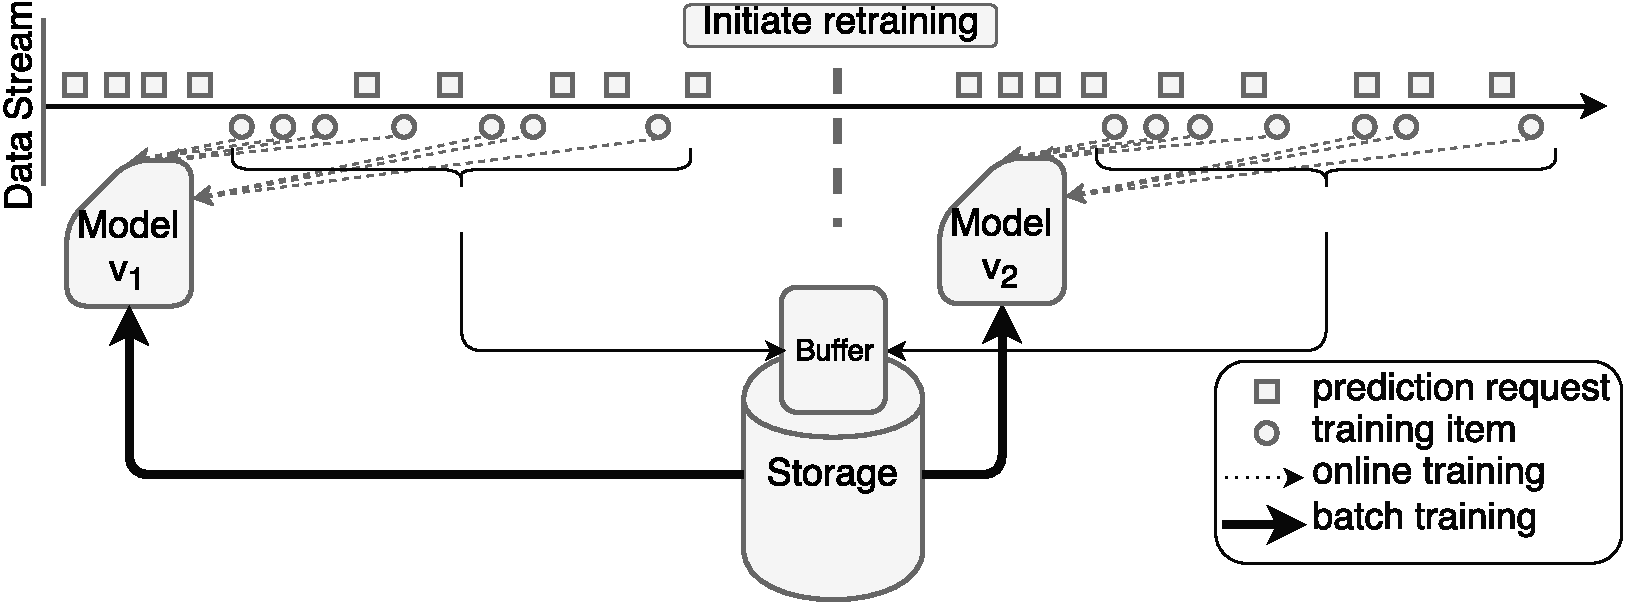
\includegraphics[width=1\columnwidth]{../images/velox-final.pdf}
\caption{Current Model Deployment Method}
\label{fig:velox-work-flow}
\end{figure}

\textbf{Example application:} to illustrate this model deployment approach, consider the task of predicting the click through rate (CTR) of online advertisements.
Search engine providers use machine learning models to estimate the expected click rate of different advertisements.
They train machine learning models based on the available data, which typically includes content of the page, search query, user information, content and meta-data of the available advertisements. 
Once such model is deployed, prediction queries of the form of ad requests arrive at the system.
The model determines the advertisements that have the highest probabilities of being clicked by the user.
Based on whether or not advertisements are clicked on, the system sends feedback in the form of new training observations, which serve to update the model accordingly.
\todo[inline]{VM:How do you make this aspect easier with your work. This is not clear to me, as this brings a batch database in, so a batch retraining might be warranted here. This might be quite different from the continuous case of periodic retraining based on new observations.
Just wondering if you convolute two things here, which may weaken your argument, as the argument of dealing with continuous observations is quite strong alone.
If you agree, I would suggest to make this aspect a secondary side-aspect, but not give it the equal prominence as the continuous retraining.

BD: My goal is to have "Introduction of new batch datasets" as a secondary goal. When a batch dataset becomes available, the system will periodically sample from it and use it in new iterations. Using this method eliminates the need for complete retraining. However, I do not perform any experiments for this specific use case. I suspect that for some datasets, the quality may be affected negatively until enough iterations of SGD using samples from the new datasets are executed. As Volker suggested, I would like to make it a secondary side-aspect/goal. Should I remove this sentence and discuss the "Introduction of new batch datasets" somewhere else, or should I remove it completely?}
Furthermore, new batch training datasets in the form of user databases, new advertisements with their metadata and more web pages will become available as more companies employ the service of the search engine provider.
\todo[inline]{VM: Is this describing the problem, or is that not already your solution? If so, this should be made clearer

BD: This is describing the current method of model deployment (using periodic retraining). Should I explain how my deployment method will help improving the use case as well? }
In order to leverage the new data and reduce the error introduced by incremental learning, the model is periodically retrained using the entire data.
Figure \ref{fig:click-rate} demonstrates the CTR prediction example for a search engine provider.

\begin{figure}[h]
\centering
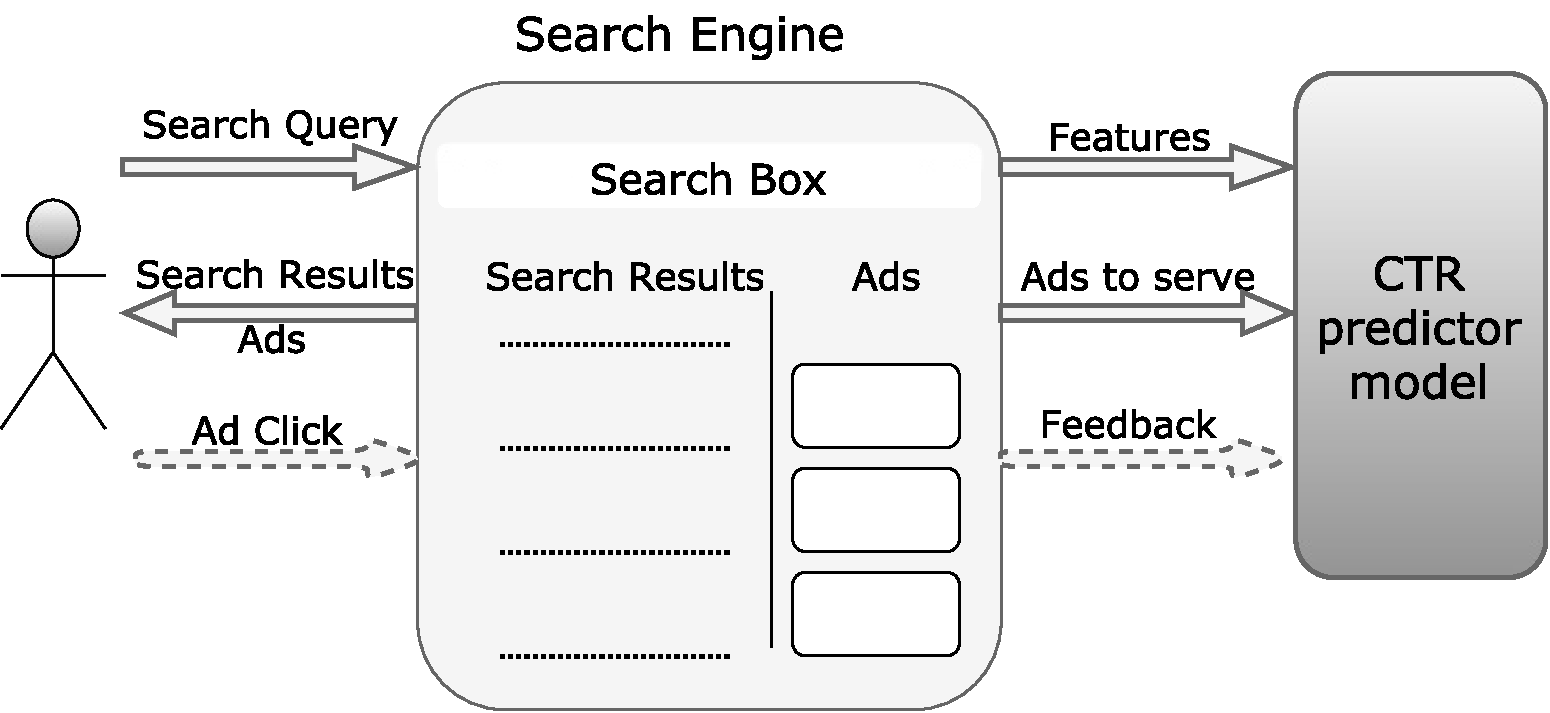
\includegraphics[width=\columnwidth]{../images/use-case-final.pdf}
\caption{Use Case: Click Through Rate Prediction}
\label{fig:click-rate}
\end{figure}

Some emerging machine learning systems have tried to automate this process \cite{crankshaw2014missing}.
They automatically deploy the model into a production environment, monitor its quality, and initiate a retraining when required.
However, they treat the underlying machine learning models as black boxes. 
As a result, they miss many opportunities for optimizing the training and deployment process.
% What is the motivation for this work
%Given the lack of systems to support model deployment and maintenance, we have set out to design a system that not only supports deployment and maintenance of machine learning models but also provides %constant crashing and batch updates while the system is running. 
%We propose the design of a system that provide 
%real-time query support as well incremental and fast batch updates to the machine learning models.

Our key observation is that, by exploiting the iterative nature of the underlying optimization algorithm, i.e., stochastic gradient descent (SGD), the model training process can be seamlessly executed with the serving and query answering component.
Based on this observation, we present a system, that supports deployment, maintenance, and incremental and fast batch updates of machine learning models.
Our contributions are as follows:
\begin{itemize}
\item We define a system for machine learning models deployment and maintenance and provide a prototypical implementation
\item We allow for incremental updates to the model, thus handling changes in the data distribution
\item We eliminate offline batch retraining and replace it with a series of single iteration of SGD
\end{itemize}
Our experiments show that our approach improves the runtime of model training and deployment by an order of magnitude over the state of the art while retaining the quality of the model. 
The speedup is due to the fact that we are able to completely eliminate batch retraining. 
Our method can also adapt to changes in the distribution faster than the existing methods.

% Outline: The rest of this document is structured as follows. ...
The rest of this paper is organized as follows. 
Section \ref {related-work} discusses related work.
In section \ref{sgd}, we describe the underlying optimization method.
Section \ref{continious-training-serving} and \ref{sec:system-architecutre} introduce the design principles and architecture of our deployment system.
In Section \ref{evaluation}, we evaluate our system against different workloads and compare the performance of our method to other model deployment and maintenance approaches. 
Finally, Section \ref{conclusion} presents our conclusion and future work.

\section{Related Work} \label{related-work}
\todo[inline]{Which one is better: training and managing .... deploying and maintaining OR training and managing ... deployment and maintenance}
Traditional machine learning systems focus solely on training and managing models and leave the task of deploying and maintaining to the users. 
It has only been recently that some systems, for example Velox \cite{crankshaw2014missing}, TensorFlow Serving \cite{abadi2016tensorflow}, and LongView \cite{akdere2011case} have proposed architectures that also consider model deployment and query answering.
LongView integrates predictive machine learning models into relational databases. 
It answers predictive queries and maintains and manages the models.
LongView uses techniques such as query optimization and materialized view selection to increase the performance of the system.
However, it only works with batch data and does not provide support for real-time queries. 
As a result it does not support incremental learning.
In contrast, our system is designed to work in a dynamic environment where it answers prediction queries in real-time and incrementally updates the model when required.
TensorFlow Serving provides mechanisms for real-time queries, deployment and version control of machine learning models.
It has out-of-the-box support for models created using TensorFlow and provides several interfaces for users to deploy their custom models.
However, it does not provide incremental updates to the model.
Contrary to our system, models have to be retrained outside of the system and have to be redeployed to TensorFlow Serving once the training is complete.
Moreover, TensorFlow is designed to create and train only deep neural network models and does not work with other machine learning models.
Our system supports incremental and batch updates to the model and automatically applies these updates to the model currently being served.
Furthermore, our system can work with any machine learning model that uses stochastic gradient descent as optimization algorithm.

Velox is an implementation of the common machine learning serving practice \cite{crankshaw2014missing}, explained in Section \ref{introduction}.
Velox supports incremental learning and can answer prediction queries in real-time.
It also eliminates the need for users to manually retrain the model offline and redeploy it again.
Velox monitors the error rate of the model using a validation set.
Once the error rate exceeds a predefined threshold, Velox initiates a complete retraining of the model using Spark. 
This deployment method, however, has three drawbacks; retraining discards updates that have been applied to the model so far, the process of retraining on full data set is resource intensive and time consuming, and new datasets introduced to the system only influence the model after the next retraining.
Our approach differs, as it exploits the underlying properties of SGD to fully integrate the training process into the system's lifeline.
This eliminates the need for completely retraining the model and replaces it with consecutive SGD-iterations.
Moreover, our system can train the model on new batch datasets as soon as they become available.

Clipper \cite{crankshaw2016clipper} is another machine learning deployment system that focuses on producing higher quality predictions by maintaining an ensemble of models.
It constantly examines the confidence of each model.
For each prediction request, it uses the model with the highest confidence.
However, it does not incrementally train the models in production, which over time leads to models becoming outdated.
Our deployment method on the other hand, focuses on maintenance and continuous updates of the models.

Weka \cite{hall2009weka}, Apache Mahout \cite{Owen:2011:MA:2132656}, and Madlib \cite{hellerstein2012madlib} are systems that provide the necessary toolkits to train machine learning models. 
All of these systems provide a range training algorithms for machine learning methods. 
However, they do not provide any management, before or after the models have been deployed. 
Our proposed system focuses on models trainable using stochastic gradient descent and as a result is able to provide model management both during training and deployment time.

MLBase \cite{kraska2013mlbase} and TuPaq \cite{sparks2015tupaq} are model management systems.
They provide a range of training algorithms to create machine learning models and mechanism for model search as well as model management.
They focus on training high quality models by performing automatic feature engineering and hyper-parameter search.
However, they only work with batch datasets.
Once models are trained, they have to be deployed and used for serving manually by the users.
Our system, on the contrary, is designed for deployment and maintenance of already trained models.

\section{Stochastic Gradient Descent} \label{sgd}
Machine learning minimizes an objective function (often referred to as the loss function).
Usually, this requires us to calculate the gradient of the function at different data points and update the function parameters based on the gradient values.
A common optimization method is gradient descent, an iterative process where each iteration uses the entire training data set to calculate the gradient value.
One drawback of gradient descent is that in presence of large datasets it performs very slow.
Stochastic gradient descent \cite{bottou2010large} is an approximation of the gradient descent method. 
Similar to gradient descent, it is an iterative process.
However, in each iteration it calculates the gradient at a single element (or a small sample) and updates the parameters of the model accordingly. 
Although it converges after a higher number of iterations, the overall convergence time is lower (sometimes by orders of magnitude) than gradient descent \cite{bottou2010large}. 
Each iteration of SGD executes in a short amount of time because it only works with a sample of the data.
We are leveraging this property of SGD and design our deployment system so that it performs one iteration of SGD at a time without interrupting the query answering component.
In Section \ref{evaluation}, we show that the overhead from executing a single iteration of SGD is very small and does not affect the query answering component.

\subsection{Distributed SGD}
To efficiently train machine learning models on large datasets, scalable techniques have to be employed.
SGD inherently works well with large amounts of data because it does not need to scan every data point during every iteration.
However, for very large datasets, SGD has to perform many iterations in order to converge.
To decrease the running time, large datasets can be distributed among multiple nodes, where each node will compute the gradients on a subset of the data in parallel.
One drawback of this approach is that a synchronization step is required before applying the updates to the model, which slows down the optimization process.
To alleviate this, several asynchronous SGD methods are proposed \cite{recht2011hogwild, dean2012large}. 
Experiments using these methods show that the quality of the produced model is similar to the synchronized SGD approach.

\subsection{Machine Learning Models based on SGD}
SGD is a common optimization methods that has been used in classification \cite{zhang2004solving}, clustering \cite{bottou1995convergence}, neural networks \cite{dean2012large}, and matrix factorization \cite{funk2006netflix}.
Some examples of machine learning models that use SGD are: 

\textbf{Linear Classifiers} are arguably the most common type of machine learning models built using the SGD optimization method. 
In the CTR prediction example of Section \ref{introduction}, we use logistic regression to train the model for predicting the click through rate \cite{macmahan2013}. 
Logistic regression models typically output a probability instead of a class label that indicates how likely an item belongs to a specific class \cite{hosmer2013applied}.
In our example, logistic regression predicts the click probabilities for all the available advertisements and the ones with the highest probabilities are displayed.
Support vector machines (SVM) represent another common class of classification models \cite{steinwart2008support}.
While logistic regression aims to find parameters of a function that accurately fit the data points to the labels, SVM tries to separate the data points belonging to different classes. 
In many cases, both types of models work equally well.
However, depending on the data (whether it is linearly separable or not) and result requirements (probability values or class labels) one method may be preferred to the other.

\todo[inline]{VM: Have you not described some of that earlier? Also, is this background really necessary for your paper?

BD: These are the methods that I have implemented in the prototype, that's why I thought I should explain them briefly.}
\textbf{Matrix Factorization} is a common method used in recommender systems \cite{koren2009matrix}. 
Matrix factorization is used to derive the latent factors (e.g., for users and items) for recommender systems.
It relies on the fact that each user and item can be described in a few dimensions (10 to 40 usually) based on the available ratings.
These latent factors automatically capture the similarity of users and items based on the ratings provided by the users.
Hence, any unknown rating can be predicted by computing the dot product of the user vector with the item vector.
A scalable version of the algorithm was proposed by Gemulla et al. \cite{gemulla2011large}.

\todo[inline]{VK: Same as previous paragraph?
Maybe can be shortened/removed?
This looks more like further related work, distracting from the "meat" of your paper

BD: Should I get rid of them completely ? }
\textbf{Neural Networks} or deep learning -- inspired by biological neural networks in the brain -- are used to learn and approximate complex functions. 
They have been used for more than half a century to model functions and have been successfully applied to training machine learning models.
However, due to the slow training process and the lack of large amount of training data, they have not been used extensively in the machine learning community in the past.
In the last decade, there was a drastic change due to several seminal publications.
Hinton et al. proposed methods for speeding up the training of neural networks \cite{hinton2006fast}.
The ImageNet competition \cite{ILSVRC15} in 2012 was won by a neural network proposed by Krizhevsky et al. where they significantly reduced the error rate \cite{krizhevsky2012imagenet}. 
The success of the Google's Deepmind team in achieving Neural Networks that were capable of defeating humans in the game of Go \cite{silver2016mastering} and mastering Atari games \cite{mnih2013playing} was also instrumental in popularizing neural networks in the machine learning community.

SGD is the ideal optimization algorithm for training neural networks since it works very well with large datasets (which are required for training neural networks).
In fact, almost all of the recent work on neural networks use SGD for training them.

\begin{figure}[t]
\centering
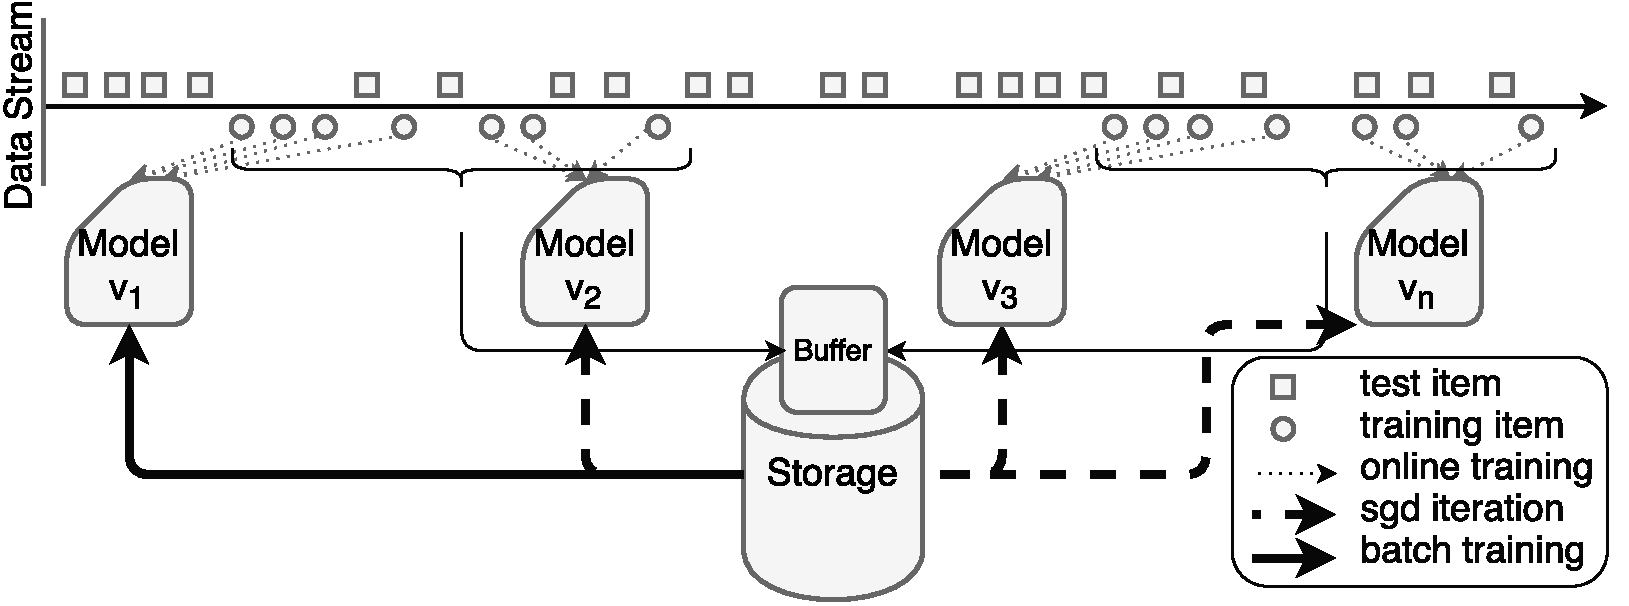
\includegraphics[width=\columnwidth]{../images/continuous-final.pdf}
\caption{Continuous Training and Serving}
\label{fig:cont-training-serving}
\end{figure}

\section{Continuous Training and Serving} \label{continious-training-serving}
\todo[inline]{VK: You should later describe how severe that limitation is. So maybe the previous text on Neural networks and Matrix Factorization is useful in this context, but rather use this to make the point that your method applies broadly and that focusing only on SGD is focusing on a practically relevant class of problems. While you describe a lot in a tutorial style, what these methods are, you do not really make this line of argument very clearly yet. It might be useful to strengthen the paper.

BD: Any suggestions how to incorporate VM's comment?}
Our proposed deployment and maintenance system uses SGD as its underlying learning algorithm.
As a result, it can update the model incrementally (one training item at a time) or use mini-batches of data (1 iteration of SGD).
The core design principles of our deployment system are threefold.
First, we incrementally update the model so that it can adapt to changes in the distribution of the incoming data.
Second, we eliminate retraining and replace it with a series of consecutive iterations of SGD.
And finally, we immediately use new batch datasets that are available to the system.
Figure \ref{fig:cont-training-serving} shows how our deployment method works.
First, using the existing data residing on disk, we train an initial model and deploy it into the system.
The system receives prediction queries and training observations in a streaming fashion.
The deployed model answers incoming prediction queries as soon as they are received.
Once the system receives a training observation it updates the model incrementally.
The system also keeps track of incoming training observations and adds them to an intermediate buffer.
A scheduler component, triggers new iterations of SGD based on the rate of incoming training observations. 
The scheduler can also decide to run an iteration when the system is not under heavy load.
Each new iteration uses a random sample of the data in storage and the data in the buffer. 
Moreover, our system stores new batch datasets in the buffer (or the persistent storage unit) as soon as they become available.
Any further scheduled iteration of SGD incorporates the new data without requiring the model to be retrained from scratch.

\section{System Architecture} \label{sec:system-architecutre}
\begin{figure}[t]
\centering
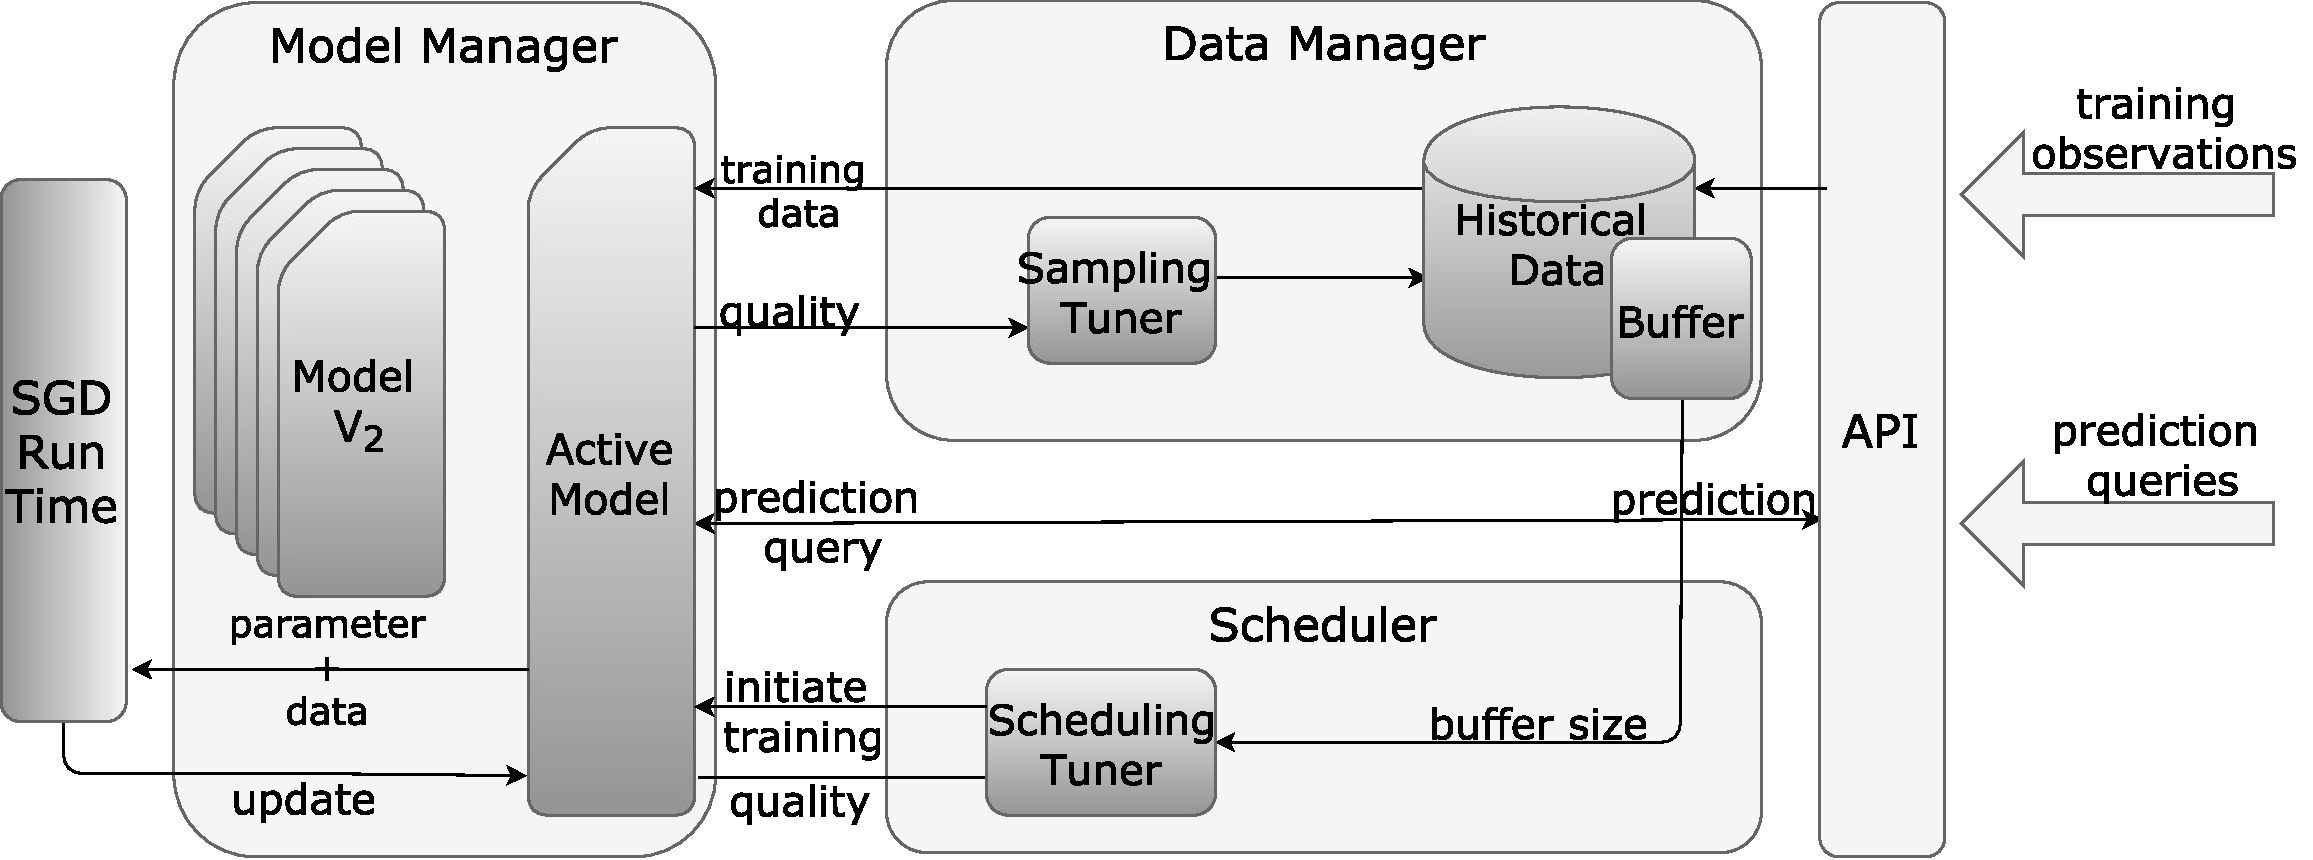
\includegraphics[width=\columnwidth]{../images/system-architecture-final.pdf}
\caption{System Architecture}
\label{fig:system-architecture}
\end{figure}

The proposed system comprises three main components; model manager, data manager and scheduler, and an independent SGD run-time. 
Figure \ref{fig:system-architecture} gives an overview of the architecture of our system and the interactions among its components.
The data manager first stores the incoming training observations in a buffer and then passes them on to the model manager.
The model manager incrementally updates the model using the training observations.
The model manager is also responsible for receiving prediction requests.
Once it receives a request, it uses the latest version of the model to make a prediction and returns the result to the user.
Both the scheduler and the data manager components are constantly communicating with each other and with the model manager, to obtain the latest statistics, such as the model quality and buffer size.
This in turn helps us to tune the scheduling and sampling rate for future iterations of SGD. 
Next, we explain each component of the system in more detail.

\subsection{Scheduler}\label{scheduler}
The scheduler component is responsible for scheduling new iterations of SGD.
Intuitively, the best time to execute an iteration is when the system is not under heavy load.
A new iteration of SGD is also executed when the system receives more training data than can be handled by the intermediate buffer.
If the model is not updated with the new training items frequently, the quality decreases.
This decrease in the quality is more rapid if the distribution of the data is changing.
In our prototype, the scheduling rate is controlled by a user defined parameter, \textit{max\_buffer\_size}.
When the intermediate buffer's size reaches \textit{max\_buffer\_size}, the scheduler executes a new iteration of SGD.
It is important to note that the scheduling rate affects the quality of the model.
In Section \ref{evaluation}, we investigate the effect of scheduling rate on model quality.
If no new training data is available, the model parameters will eventually converge and any further training iterations will not have any effect on the model quality.
Therefore, the scheduler component has to communicate with the model manager in order to detect whether the model parameters have converged and stop further iterations until more training data becomes available.

\subsection{Data Manager} \label{data-manager}
In order to execute an iteration of SGD, we need to combine the training data that arrives at the system in real-time with the data stored on disk.
The data manager is responsible for storing the incoming training observations in an intermediate buffer.
Upon a new training iteration, the data manager accesses the historical data stored on disk and provides a sample.

Different sampling strategies can be used to provide the sample.
In our current prototype, the data manager uses a simple unified random sampling method to generate this sample.
More advanced methods, such as Reservoir \cite{vitter1985random} or weighted random sampling can also be used to generate the sample.
Reservoir sampling is typically used to generate samples from large datasets that do not fit in memory, whereas weighted random sampling is used when data elements have different weights.
In an online machine learning scenario, recent items are more important for training the model and are assigned a bigger weight than older items.
Therefore, weighted random sampling can generate samples that can contribute to the training of a better model.

The data from the sample and the data in the buffer are merged to create the dataset for next training iteration.
The data manager provides access to this dataset for the model manager in order to further train the model.
The data manager also communicates with the scheduler in order to inform it when the intermediate buffer is becoming full and a new training iteration is required. 

The created data set consists of the data inside the buffer and a sample of the historical data as described earlier.
The sampling rate is a system parameter that has to be configured.
It can be pre-configured to a constant value based on the application.
However, using the feedback from the system's model manager (Section \ref{model-manager}), the sampling rate can be adjusted.
For example, when the data distribution is changing, a smaller sampling rate places more emphasis on the data that arrived recently. 
This is similar to the problem of concept drift where the distribution of the incoming data changes overtime.
This renders historical data less important and as a result a smaller sample of the historical data (or none at all) will give more importance to the data in the buffer and help the model to adopt faster to the concept drift.
However, if there is no concept drift in the data, a larger sampling rate will increase the quality of the model after a training iteration.
Another effect that the sampling rate has on the system is the training iteration running time.
A larger sampling rate increases the running time of each training iteration as more data has to be processed.
In Section \ref{evaluation}, we investigate the effects of different sampling rates on both the quality and performance of the system.

Moreover,  new data sets can be registered in data manager.
In our current prototype, new data sets first have to be stored on disk, and data manager can be informed of the data path.
Newly available data sets are used in the subsequent SGD iterations.

\subsection{Model Manager} \label{model-manager} 
An important part of the system is the model manager component.
It is responsible for storing the model, answering prediction queries, and performing incremental and batch updates to the model.
Listing \ref{model-manager-api} shows the API of the model manager.
The API is used to interact with other components as well as end-users of the system.
The scheduler component uses \textit{update} and \textit{update\_iteration} to instruct the model manager to perform incremental or batch updates (one iteration of SGD) to the model.
Upon a new prediction query, the \textit{predict} method is called to provide the end-user with the label of the given input.

\noindent\begin{minipage}[t]{\linewidth}
\begin{lstlisting}[language=java, basicstyle=\small\ttfamily, frame=tb ,columns=fullflexible,
showstringspaces=false,label=model-manager-api,caption=Model Manager API, numberstyle=\tiny]
def update(x,y)

def update_iteration(X,Y)

def predict(x): Label

def error_rate(X_test, Y_test): Double

\end{lstlisting}
\end{minipage}


The \textit{error\_rate} method returns the error rate of the model using the provided test dataset.
As described earlier, constant monitoring of the quality is required in order to adjust the scheduling and sampling rate.
When the error rate is stagnating, the model has converged using the existing data.
Therefore the model manager informs scheduler not to schedule any new iterations until new training observations have arrived at the system.
Similarly as explained in Section \ref{data-manager}, an increase in the error rate may indicate a change in distribution of the data.
As a result, reducing the sampling rate will place more emphasis on recent data (in the intermediate buffer) and help adapt the model to the changes in the distribution.

The model manager also keeps track of the changes that are made to the model.
The model is updated both through incremental learning and SGD-iteration.
The model manager creates snapshots of the model in two different scenarios; after a series of incremental updates are made and after each training iteration.
This versioning of the models is essential.
When there is a rapid change in the distribution of the incoming data (a sudden concept drift) or when there are anomalies in the data, it is sometimes necessary to revert back to a version before the change in distribution occurred.
In case of concept drift, new training iterations should be scheduled that only use the data in the buffer.
Moreover, in case of anomalies in the data, they have to be identified and discarded before any further model updates could happen.

\subsection{SGD Run-Time} 
All components of our model serving system described so far are not limited to any specific run-time.
We have decoupled the components from the actual run time of the system.
Any system capable of performing incremental and batch SGD updates efficiently are suitable options for our system.
Apache Flink \cite{carbone2015apache} and Apache Spark \cite{zaharia2010spark} are distributed data processing platforms that work with data in memory and have support for iterative algorithms, which makes both of them ideal options for our SGD run-time.
In our current prototype, we are using Apache Spark \cite{zaharia2010spark} as our SGD run-time.

The model manager is the component responsible for communicating with the SGD run-time.
In the current version of our prototype, the model manager requests Spark to perform both incremental and batch updates to the model.
Both types of updates are supported by the built in machine learning library of Spark.
The choice of run-time for SGD slightly influences the data manager as well.
In our prototype, historical data is stored on the Hadoop Distributed File System (HDFS) \cite{shvachko2010hadoop}.

\section{Evaluation} \label{evaluation} 
In this section we evaluate the performance of our system using various datasets. 
We report both the quality (error rate) and performance of our proposed method. 

\subsection{Setup}\label{subsec:setup}
\textbf{Environments:} We evaluate our deployment method on two environments; local and distributed.
We use a single node OS X machine with  a quad-core Intel i7 and 16 GB of RAM for our local experiments.
The distributed environment consists of 11 nodes (1 master, 10 slaves).
Each node is running on a Intel Xeon 2.40 GHz 16 core processor and has 28 GB for dedicated memory for running our prototype.

\textbf{Prototypes:} we implemented two versions of our deployment method.
Version 1 is implemented using python and uses some of the libraries available in scikit-learn \cite{sklearn_api}.
This version is designed to work on a local environment.
It gives a greater control over tuning the parameters of the system, since we are able to perform incremental updates one item at a time (as opposed to Spark's micro-batching).
Version 1 supports neural networks (multi-layer perceptron) and recommender system (matrix factorization).
Version 2 is implemented on top of Apache Spark \cite{zaharia2010spark}.
It is using the SGD class of Spark's machine learning library, to execute the initial and incremental training.
Version 2 works in both local and cluster environment and supports different types of linear models (SVM, Logistic Regression and Linear Regression).

\begin{table}\centering
\begin{tabular}{lrrr}
 \toprule
Name & \#Users & \#Items & \#Ratings
\\\midrule 
Movie Lens 1M  & 6000 & 4000 & 1000000 \\
Movie Lens 100k & 1000 & 1700 & 100000 
\\\bottomrule 
\end{tabular}
\caption{Recommender System Datasets}
\label{table:recommender-systems}
\end{table}

\begin{table}\centering
\begin{tabular}{lrr}
 \toprule
Name & \#Features  & \#Instances 
\\\midrule 
Higgs  & 28 & 11000000 \\
URL Reputation & 3231961 & 2396130 \\
Cover Type & 52 & 581012 \\
MNIST & 784 & 60000 \\
SEA & 3 & 60000 \\
Adult & 123 & 48882
\\\bottomrule 
\end{tabular}
\caption{Classification Datasets}
\end{table}

\textbf{Datasets:} we use two different types of datasets in our experiments.
To evaluate the recommender system we use Movie Lens datasets, which are a collection of movie ratings \cite{harper2016movielens} .
We use two versions of this dataset (100k and 1M), each with varying number of users, movies and ratings.
Table \ref{table:recommender-systems} shows the details of Movie Lens dataset.
We have sorted the Movie Lens data set based on the ratings timestamp and items are examined one by one according to their timestamp.
This is to evaluate how each of the implemented methods react to changes in the distribution of the data.
For these two datasets, we use an evolving test set to evaluate the performance of the deployment methods.
To create the evolving test set, first we draw indices for the test items uniformly at random from the entire data.
We start with an empty test set, when we reach the index of a test item, we add that to the current test set and calculate the error rate based on the current test set (We call this a test increment).
For Movie Lens 100k, the total size of the test set is 5,000 and for Movie Lens 1M, it is 50,000. 
Each error calculation, as a result, captures the degree to which the models are adopting to the changes in the dataset.

To evaluate the classifier, we use a collection of classification datasets (mostly from UCI Machine Learning Repository\footnote{\url{http://archive.ics.uci.edu/ml/}}).
Higgs \cite{baldi2014searching} is a physics datasets which is produced using Monte Carlo simulations.
For these two datasets, the task is to distinguish between a signal process that produces a target particle (Higgs bosons) and a background process which does not.
Cover Type \cite{collobert2002parallel} is a dataset used for predicting forest cover types from cartographic variables.
We use a binary class version of this dataset\footnote{\url{https://www.csie.ntu.edu.tw/~cjlin/libsvmtools/}}.
URL Reputation \cite{ma2009identifying} is a collection of URLs and the task is to identify malicious URLs. 
This dataset is collected over 120 days and features are anonymized, but correspond to lexical and host-based information gathered for each URL.
MNIST \cite{lecun-mnist} is a dataset of handwritten digits.
Each image has 28x28 pixels and the labels are the 10 digits (0 to 9) the images are representing.
SEA is an artificially generated dataset that has been injected with concept drift (change in data distribution)\cite{street2001streaming}.
Attributes are floating point values between 0 and 10 and there are a total of 4 concepts (15,000 instances in each concept).
Adult \cite{platt199912} is a dataset extracted from a census database.
It contains information such as education level, occupation, relationship status, and salary of individuals from multiple countries and the task is to predict whether an individual earns more than \$50K a year. 
For all of the datasets we use 10\% for initial training and 90\% for online prediction/training.
Except for URL Reputation and Movie Lens datasets that are timestamped, the order of the incoming data are arbitrary for the rest of the datasets.
For all of the classification datasets, we report the prequential error \cite{gama2009issues} when receiving a new training instances.
%\textbf{Criteo \cite{criteo-kaggle}}: to implement our CTR prediction example we use Criteo's Kaggle advertising challenge dataset.
%The dataset includes both categorical and numerical features.
%However, in our evaluations we only used the numerical features.
%Similar to MovieLens datasets, we use 10\% of the data for initial training and the rest is streamed to the system.
%The training data consists of a sample of Criteo's traffic over a period of 7 days.
%We use prequential evaluation \cite{gama2009issues} to calculate the misclassification rate of the implemented deployment methods.

\textbf{Deployment methods:} In this section, we briefly describe the methods we have implemented.

\textbf{Baseline} is the naive and simplest deployment model. 
After a model is a trained from the initial data, it is used throughout the lifetime of the application without any incremental or batch learning.

\textbf{Baseline+} is similar to the baseline approach with the added incremental learning.
After the initial model is deployed, it is constantly updated based on new training items that arrive at the system.

\textbf{Velox} is an implementation of the common deployment scenario described in Section \ref{introduction}.
It is based on the the proposed system by Crankshaw \cite{crankshaw2014missing}. 
After the initial model is deployed, the model is incrementally updated with every new training item.
A full retraining of the model is performed once a certain amount of training observations have been received.

\textbf{Continuous} is the implementation of our proposed method. 
Similar to Velox and Baseline+ once, an initial model is first trained using the existing data.
New training data is used to incrementally update the model.
Based on the rate of incoming training data, a scheduler component triggers new iteration of SGD.
The data used in this new iteration of SGD consists of the new data that arrived in the system since the last scheduled iteration plus a sample of the existing historical data.

\subsection{Implementation of ML Models}
We have implemented three different machine learning models to evaluate our deployment method.
In this section, we briefly explain each of the implemented methods.

\textbf{Recommender system:} we implement a recommender system based on the matrix factorization using SGD \cite{funk2006netflix}.
Based on our initial experiments, we set the number of latent factors to 40.
First, we train a model using the initial static data.
To produce more accurate predictions, we include user, item, and global bias values as described by Simon Funk \cite{koren2009matrix}.
After the initial training, we deploy the model and use the new training observations to incrementally update the model.
Training observations are of the form \textit{\((user\_id, item\_id, rating\))}.
Based on the training observation, the bias values as well as the factors are updated for the specified user and item.

\textbf{SVM Classifier:} we implement a simple SVM classifier by extending the existing SVM classifier of Apache Spark.
We implement the necessary methods described in Section \ref{sec:system-architecutre} for the SVM classifier to work with our deployment method.
The extra methods are \textit{update} which takes one (or a micro-batch in Spark Streaming) item and incrementally update the model and \textit{update\_iteration} which takes a dataset and executes one iteration of SGD on the given data.

\textbf{Neural Network:} to evaluate our system on an image classification task, we implement a multi-layer perceptron neural network using back propagation \cite{collobert2004links}.
We set the number of hidden layers to 50 and use a softmax output function \cite{bishop2006pattern}.
Similar to recommender system case, a network is first trained on the static data.
The training observations are of the form of \textit{\((X,y)\)}, where X is a vector of 784 dimension (1 for each pixel) and y is the digit the image is representing.

\subsection{Tuning parameters} \label{tuning}
In Section \ref{continious-training-serving}, we discussed how system parameters such as sampling and scheduling rate affect the performance and quality of the system.
In this section, we analyze the effects of different sampling and scheduling rates on the system.
Our goal, is to make these parameters adaptive, but for now we analyze their effects on the running time and quality. 

\textbf{Scheduling rate:} this parameter specifies how often a new iteration of SGD should be scheduled. 
In our prototype, the scheduling rate is governed by a parameter called buffer size, which dictates how many new items should be stored in the buffer before a new iteration of SGD is executed. 
Ultimately, the system should make the decision to schedule new iterations based on the availability of resources.
Executing one iteration of SGD even using the entire data is not a resource heavy process, and can easily be done in parallel with the serving component of the system. 
This results in a paradigm where both training and serving can happen simultaneously. 

\begin{figure}[h]
\begin{subfigure}{\columnwidth}
\centering
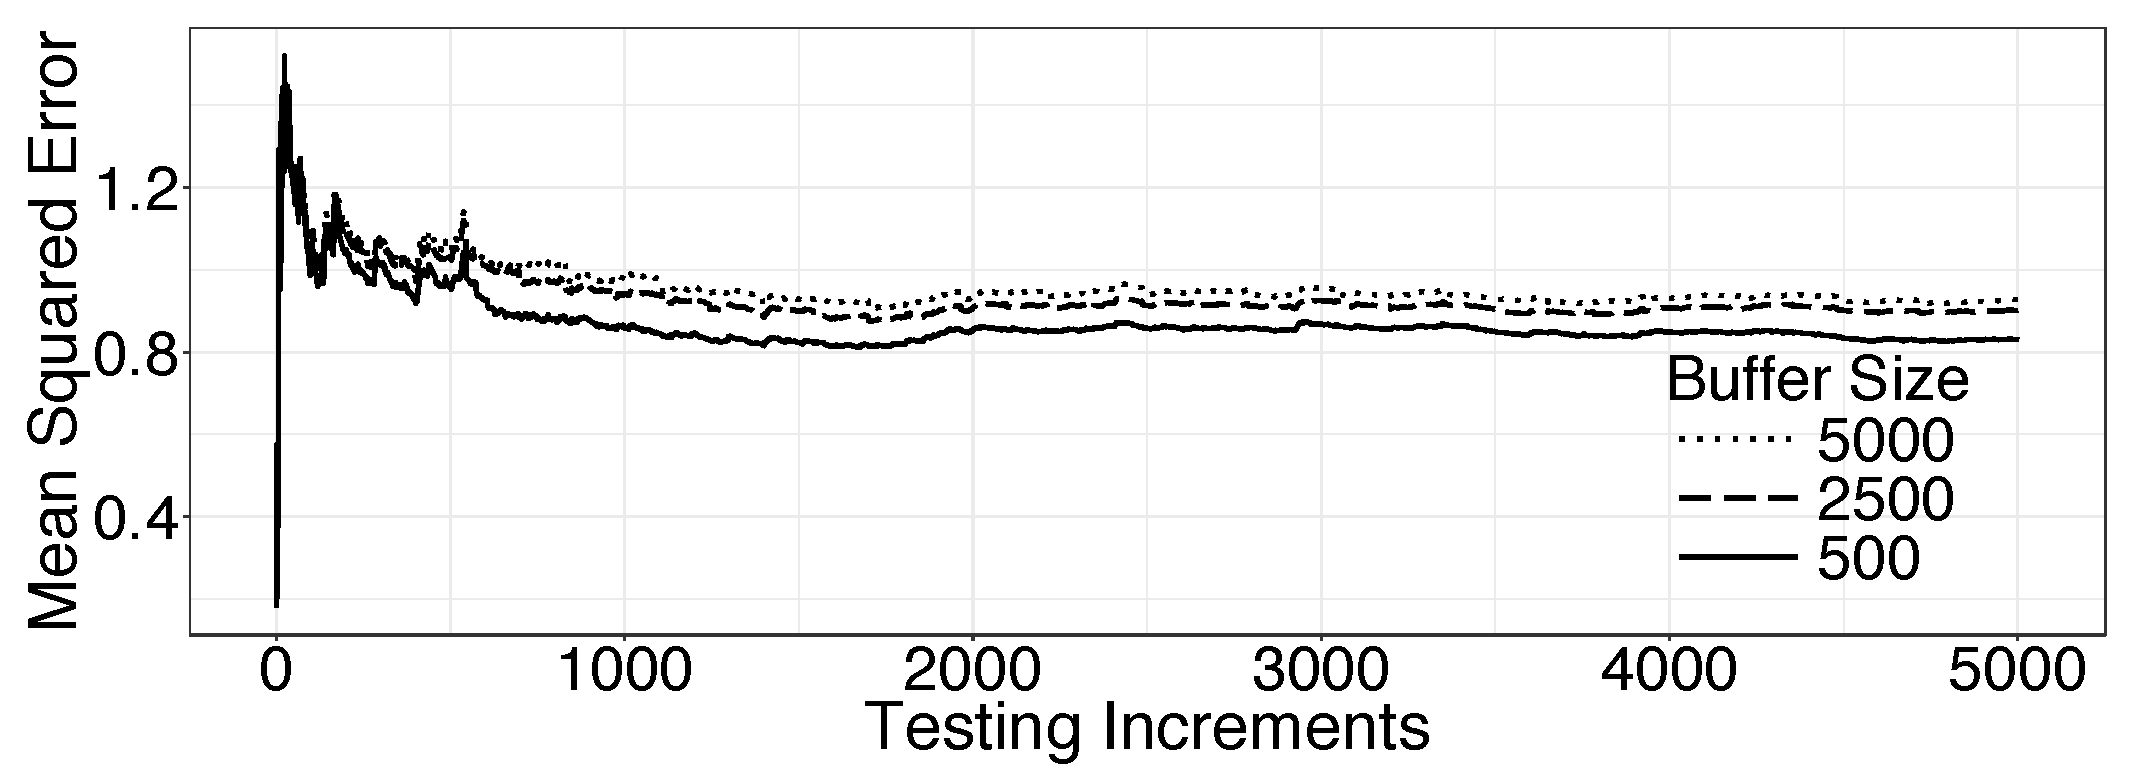
\includegraphics[width=\columnwidth]{../images/experiment-results/movie-lens-buffer-quality-improved.eps}
\caption{Buffer size}
\label{fig:movie-lens-100k-buffer-size-mse}
\end{subfigure}
\begin{subfigure}{\columnwidth}
\centering
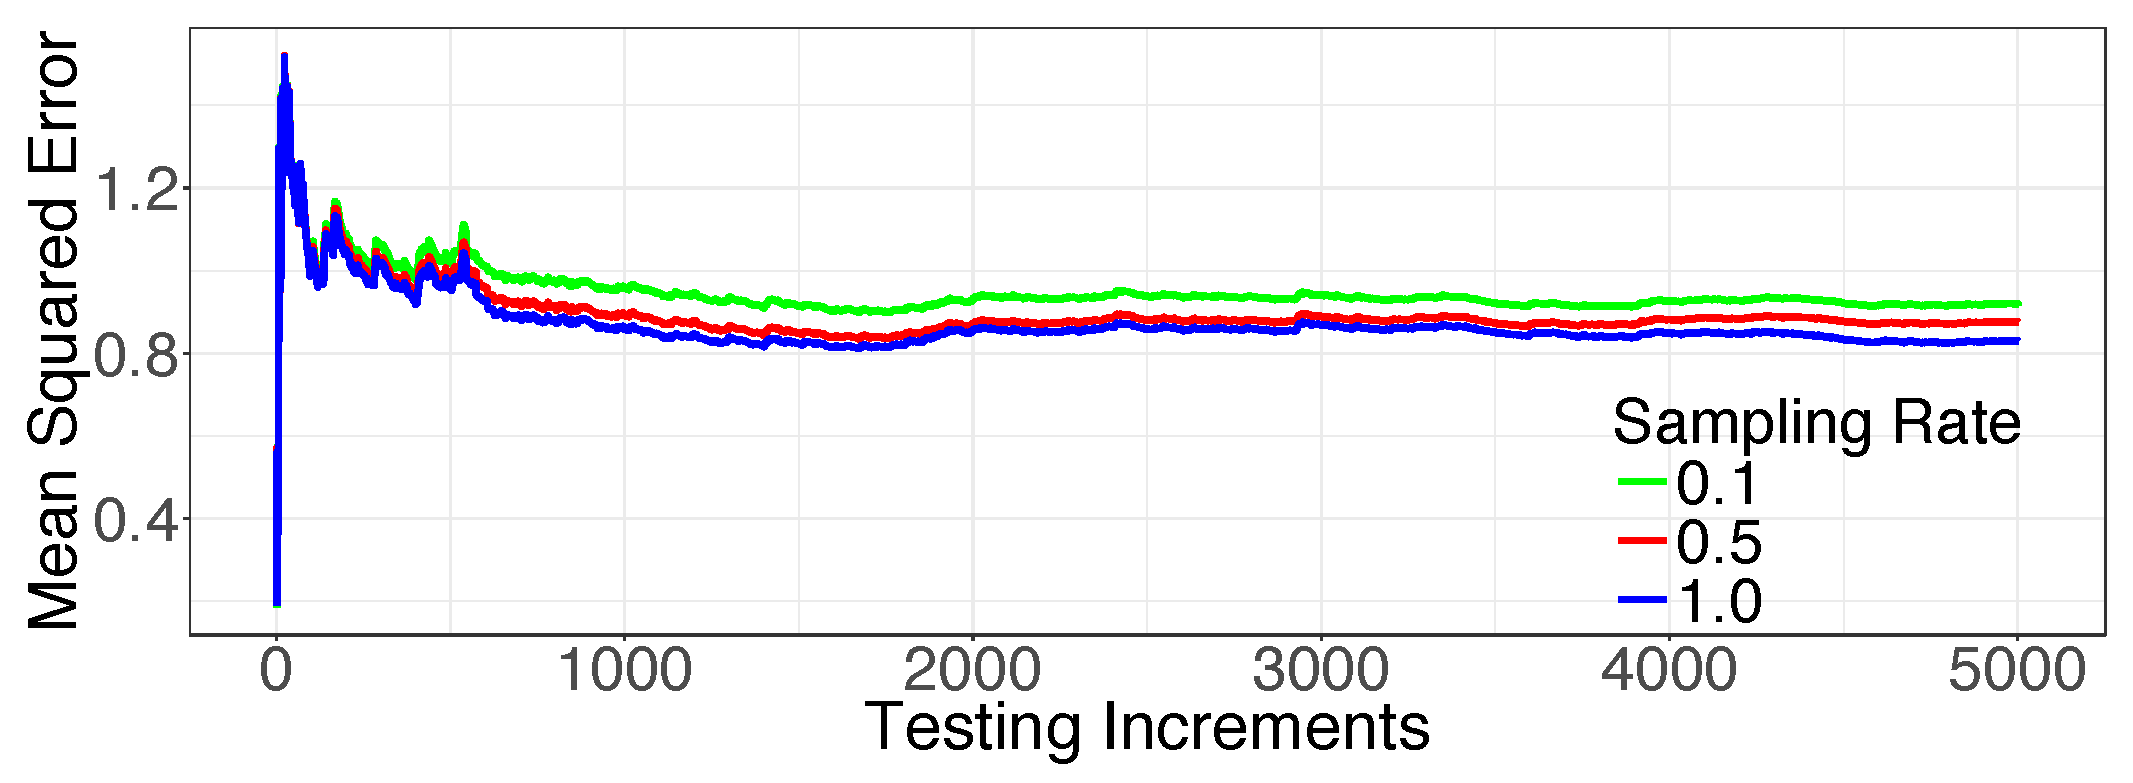
\includegraphics[width=\columnwidth]{../images/experiment-results/movie-lens-sampling-quality-improved.eps}
\caption{Sampling rate}
\label{fig:movie-lens-100k-sample-rate}
\end{subfigure}
\vspace{2mm}
\caption{Parameters effect on quality (Movie Lens 100K)}
\end{figure}

Figure \ref{fig:movie-lens-100k-buffer-size-mse} shows the mean squared error for different buffer sizes for Movie Lens 100k dataset. 
A smaller buffer size causes the scheduler to initiate training iterations more frequently.
As a result, the system updates the underlying model more frequently.
However, the error rate is not decreasing linearly with the buffer size.
Further analysis show that the more frequent the model updates are, the faster the model converges and any further training has little to no effect on the overall quality.
Therefore, increasing the scheduling rate only decreases the error rate up to a point, after which increasing the scheduling rate has no effect on the overall quality of the model.
This is extremely important, specially when considering the effect the buffer size has on the running time.
Figure \ref{fig:movie-lens-100k-buffer-size-time} shows the running time on Movie Lens 100k dataset using different buffer sizes. 
Increasing the buffer size from 500 to 5000 decreases the running time by a factor of 5 while as described before the error rate is only increased slightly.
Therefore, depending on the application, we can set the buffer size to bigger values in order to increase the performance of the system without affecting the quality of the final model substantially.

\begin{figure}[H]
\begin{subfigure}{0.5\columnwidth}
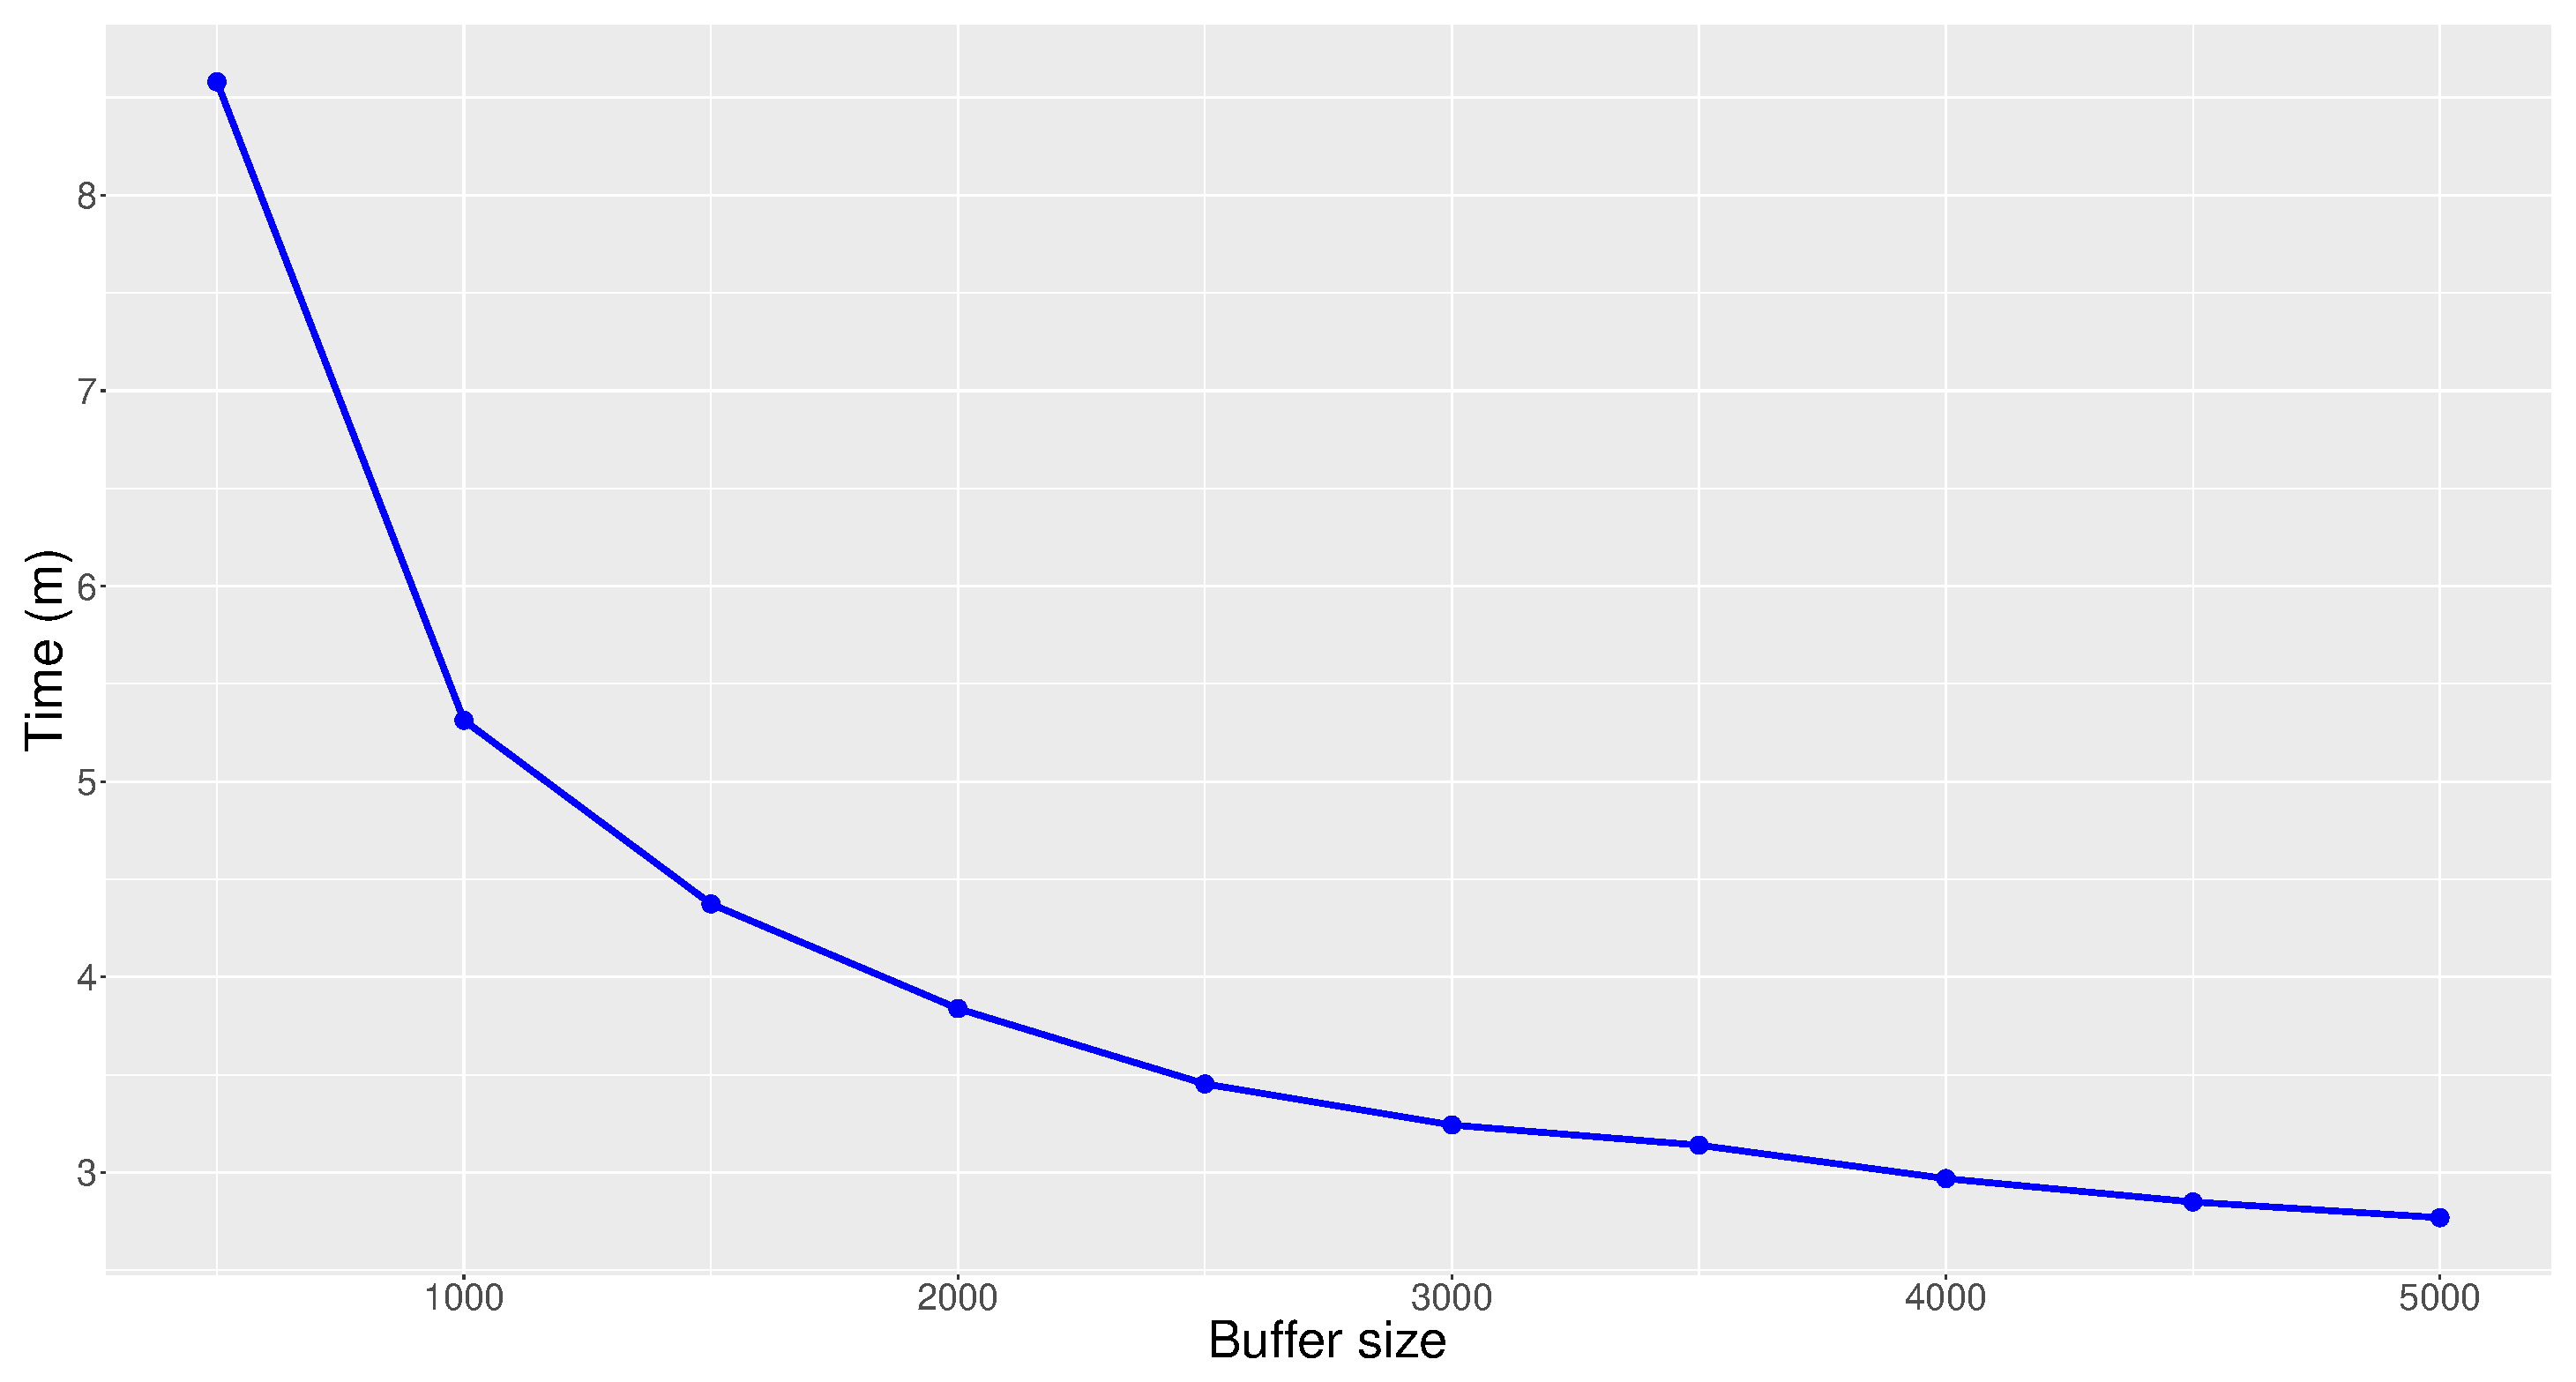
\includegraphics[width=\columnwidth]{../images/experiment-results/movie-lens-100k-buffer-time-improved.eps}
\caption{}
\label{fig:movie-lens-100k-buffer-size-time}
\end{subfigure}%
\begin{subfigure}{0.5\columnwidth}
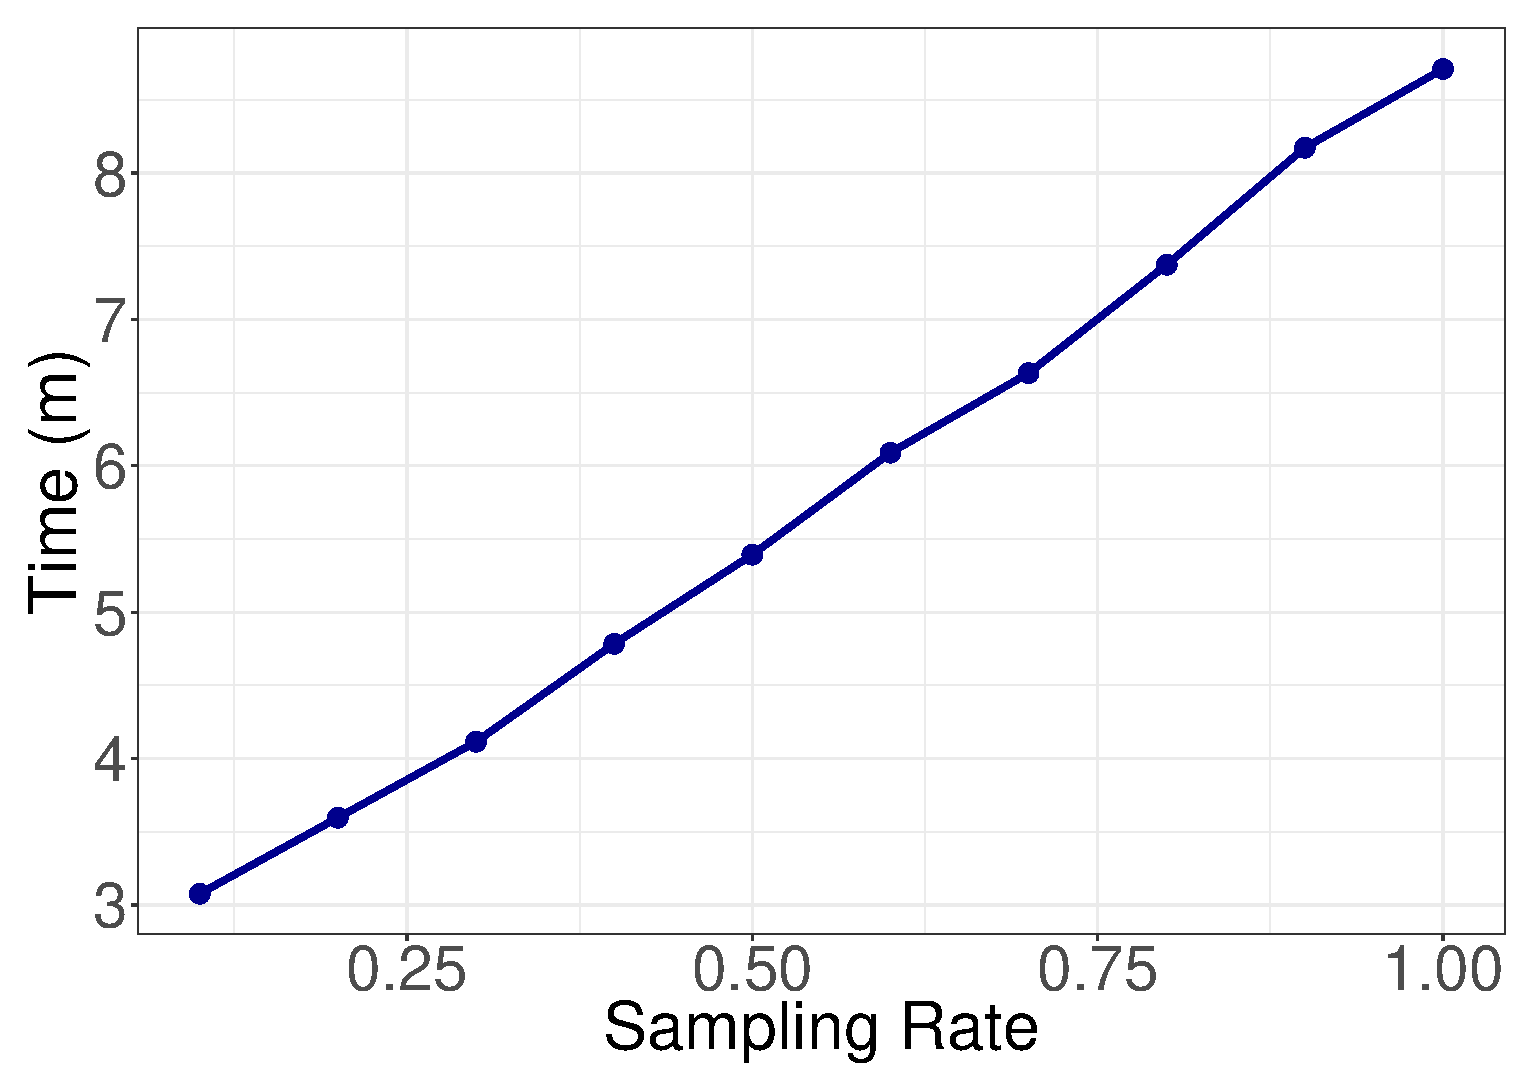
\includegraphics[width=\columnwidth]{../images/experiment-results/movie-lens-100k-sampling-time-improved.eps}
\caption{}
\label{fig:movie-lens-100k-sample-rate-time}
\end{subfigure}
\vspace{2mm}
\caption{Parameters effects on run time}
\end{figure}

\textit{Dynamic scheduling:} in production environments, the load on the system typically varies throughout the lifetime of the application.
Therefore, a dynamic scheduling maximizes the performance of the system, by performing more frequent updates while there are more resources available for training. 
Moreover, since training and serving can be done in parallel, we can perform training in the background and only update the weights when the training iteration is over. 

\textbf{Sampling rate:} in each iteration of SGD, as described in Section \ref{continious-training-serving}, the data inside the buffer and a sample of the historical data is used to update the model.
In this section, we investigate the effect of the sampling rate on the model quality and the running time of the system.
Figure \ref{fig:movie-lens-100k-sample-rate} shows that a larger sampling rate increases the quality of the model, but similar to scheduling rate, the decrease in error rate is negligible considering the effect it has on running time. 
This is again, caused by the same phenomena, where the model after training on bigger sample rates start to converge faster and as a result bigger sample sizes do not have an effect on the quality.
 
Figure \ref{fig:movie-lens-100k-sample-rate-time} shows the effect of increasing sampling rate on running time.
Using the entire historical data (sampling rate = 1.0) increases the running time 5 fold. 
Therefore, similar to the scheduling rate, setting the sampling rate to smaller values will increase the performance substantially, while only slightly affecting the quality of the model.

\textbf{Tuning parameters based on error rate:} the underlying machine learning model and the dataset have big effects on the selection of sampling rate and scheduling rate.
In the recommender system use case, due to changes in incoming data distribution, we see that bigger sample rates and higher scheduling rates have an effect (although small) on the quality of the model.
This, however, is not be the case for every application.
To demonstrate this, we perform the same set of experiments on the MNIST dataset.
Figure \ref{fig:mnist-sample-rate} shows the effect of different sampling rates on the neural network classifier model for MNIST data.
Contrary to the results we achieved for Movie Lens 100k the error rates for different sampling rates are very similar.
This is caused by how neural networks behave.
Increasing the sampling rate causes similar data items to be used repeatedly in consecutive training iterations.
Neural networks are not affected by this oversampling, therefore the results are almost similar with different sampling rates.
Moreover, in this experiment, the number of parameters of the multi-layer perceptron is far less than the number of parameters of the matrix factorization model for Movie Lens 100k.
This causes the neural work to converge faster and, therefore it is not affected by more training, unless new training observations arrive at the system.
\begin{figure}[h]
\begin{subfigure}{\columnwidth}
\centering
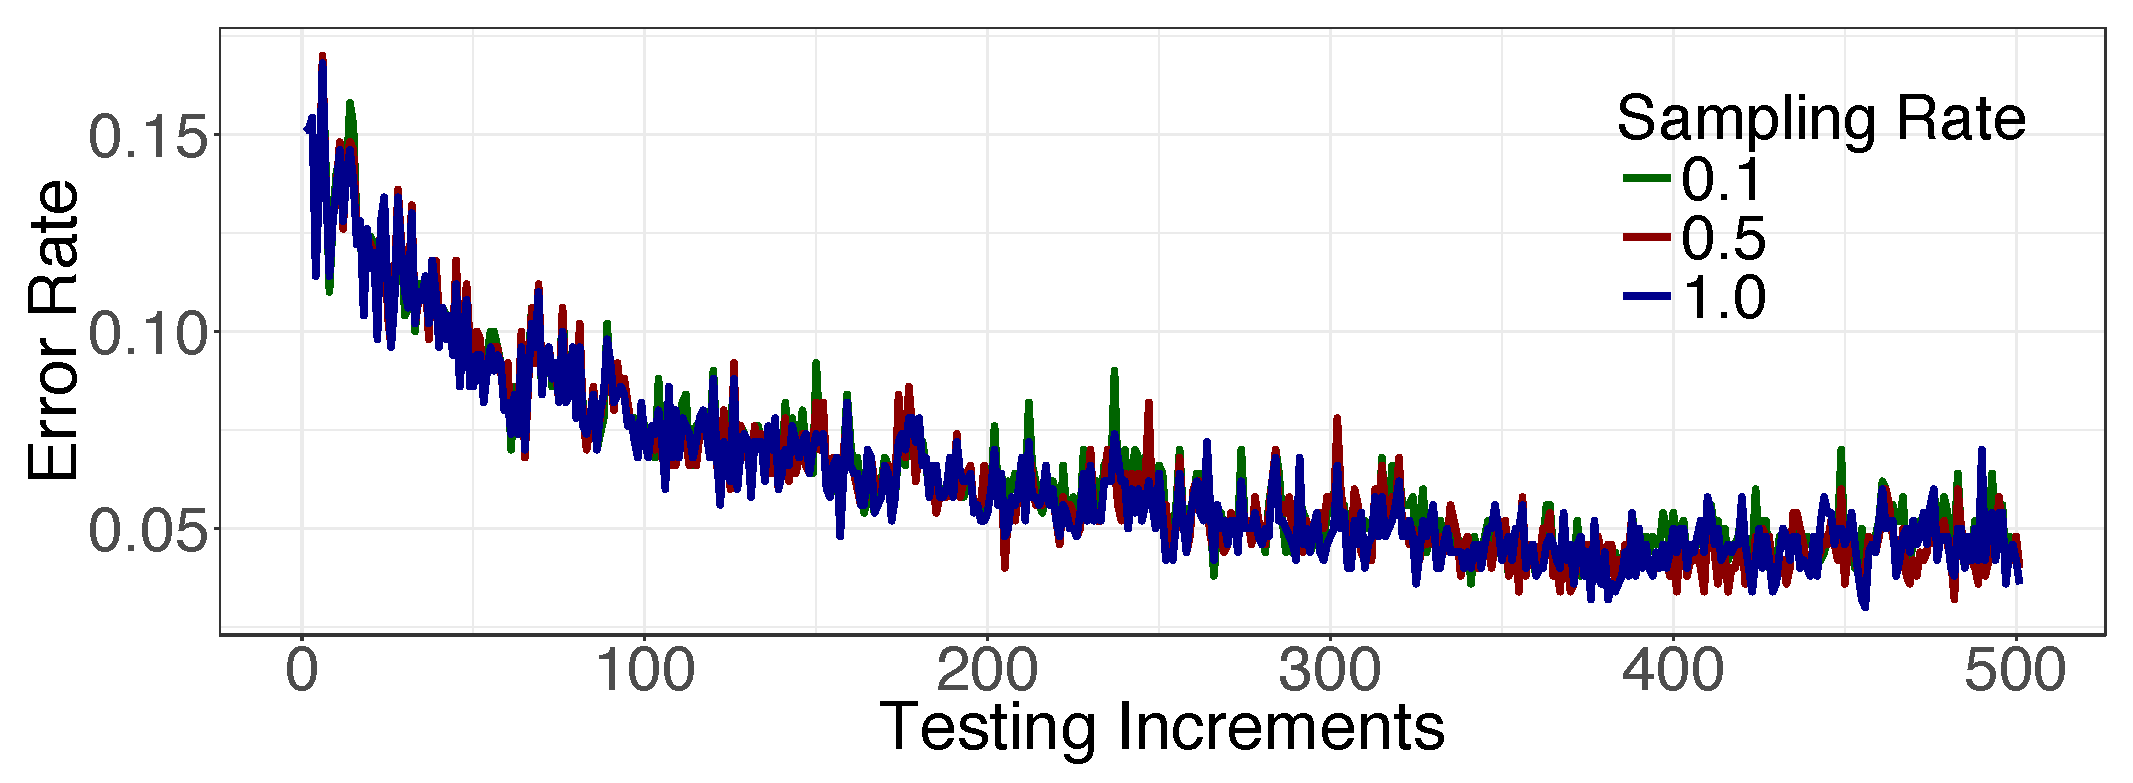
\includegraphics[width=\columnwidth]{../images/experiment-results/mnist-sampling-improved.eps}
\caption{Sampling rate}
\label{fig:mnist-sample-rate}
\end{subfigure}
\begin{subfigure}{\columnwidth}
\centering
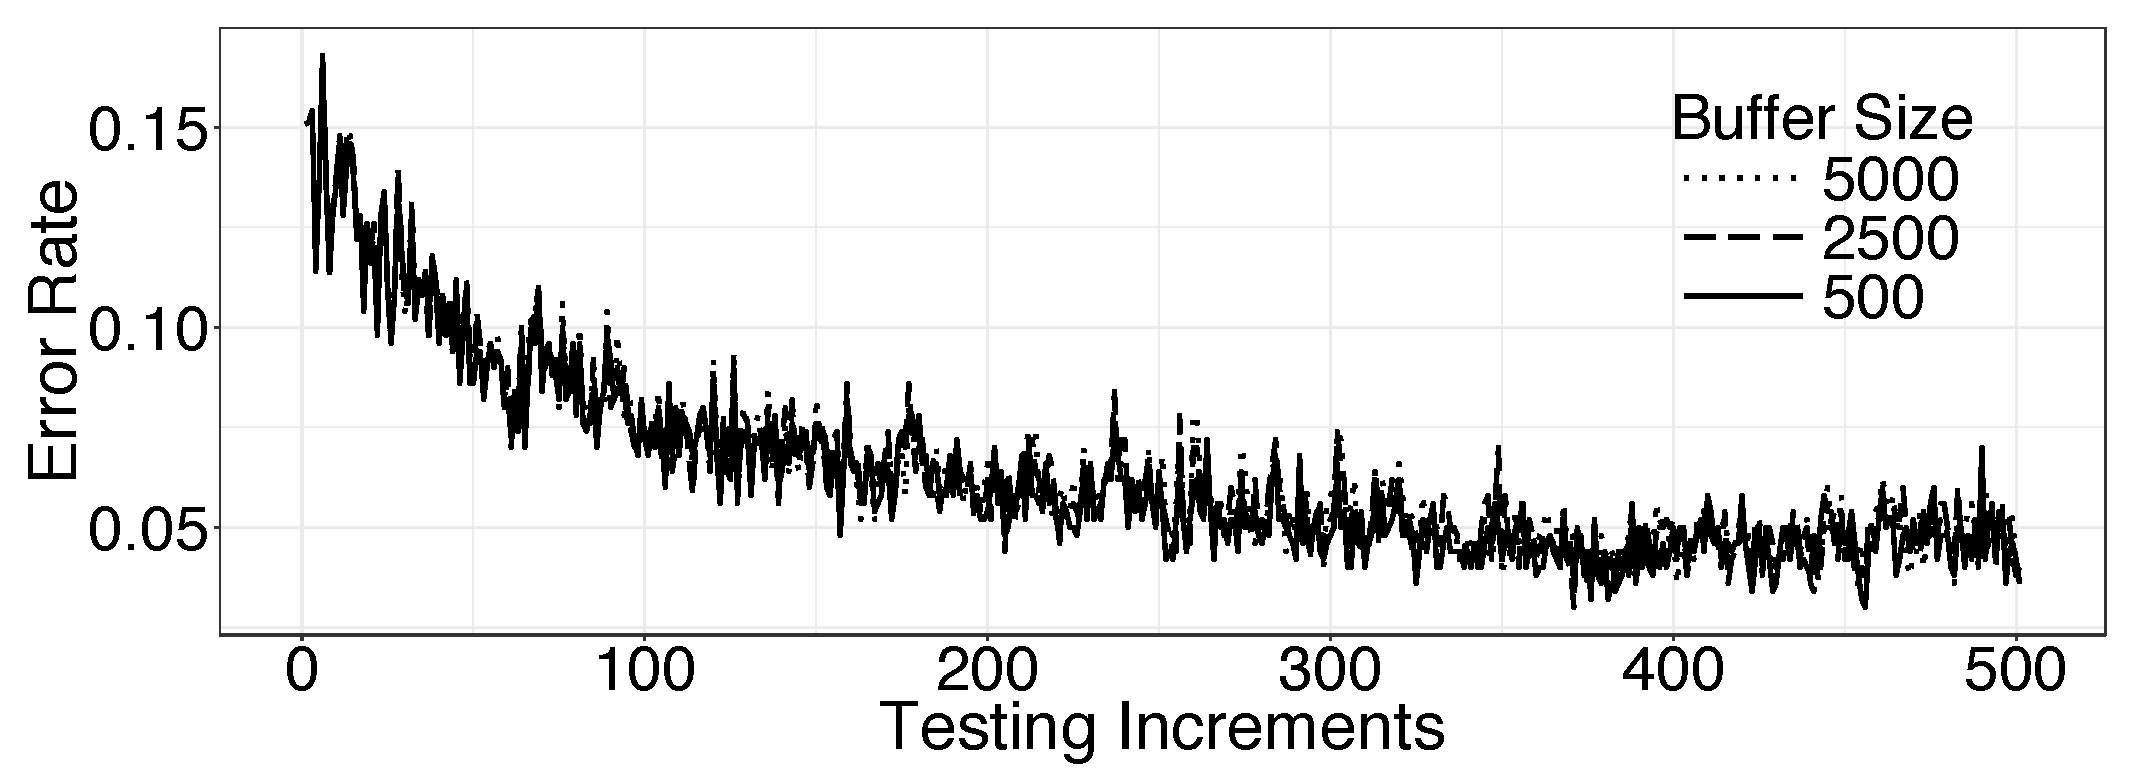
\includegraphics[width=\columnwidth]{../images/experiment-results/mnist-buffersize-improved.eps}
\caption{Buffer size}
\label{fig:mnist-buffer-size}
\end{subfigure}
\vspace{2mm}
\caption{Parameters effect on quality (MNIST)}
\end{figure}

Figure \ref{fig:mnist-buffer-size} shows how the buffer size affects the overall quality of the neural network model.
Similar to the sampling rate case, the error rates of the models are not affected by the scheduling rate.
New training observations that exist in the buffer have the maximum effect on the quality of the model since they are becoming available to the model for the first time.
As the scheduling rate increases, the number of new training observations remain the same, and only the historical data is used more frequently to train the model.
Since neural networks do not gain much benefit by revisiting the same items, increasing the scheduling rate has no effect on the overall quality.

Based on our findings, we conclude that increasing the sampling and scheduling rate does not always affect the quality.
In both the Movie Lens 100k and MNIST use cases the change in scheduling and sampling rate has small to no effect on the overall quality.
However, the running time of the methods are heavily influenced by these parameters.
Setting these parameters to small values decreases the running time considerably and save computation resources regardless of the type of model the system is serving.

\subsection{Experiments in the Local Environment}\label{subsec:experiment-local}
We evaluated our deployment method on the datasets described in Section \ref{subsec:setup}.
Our prototypes support two different methods of specifying the scheduling rate; buffer size and scheduling period.
For recommender system experiments we use the buffer size to specify the scheduling rate (in Velox's case scheduling rate corresponds to offline retraining frequency).
\begin{figure}[h]
\begin{subfigure}{\columnwidth}
	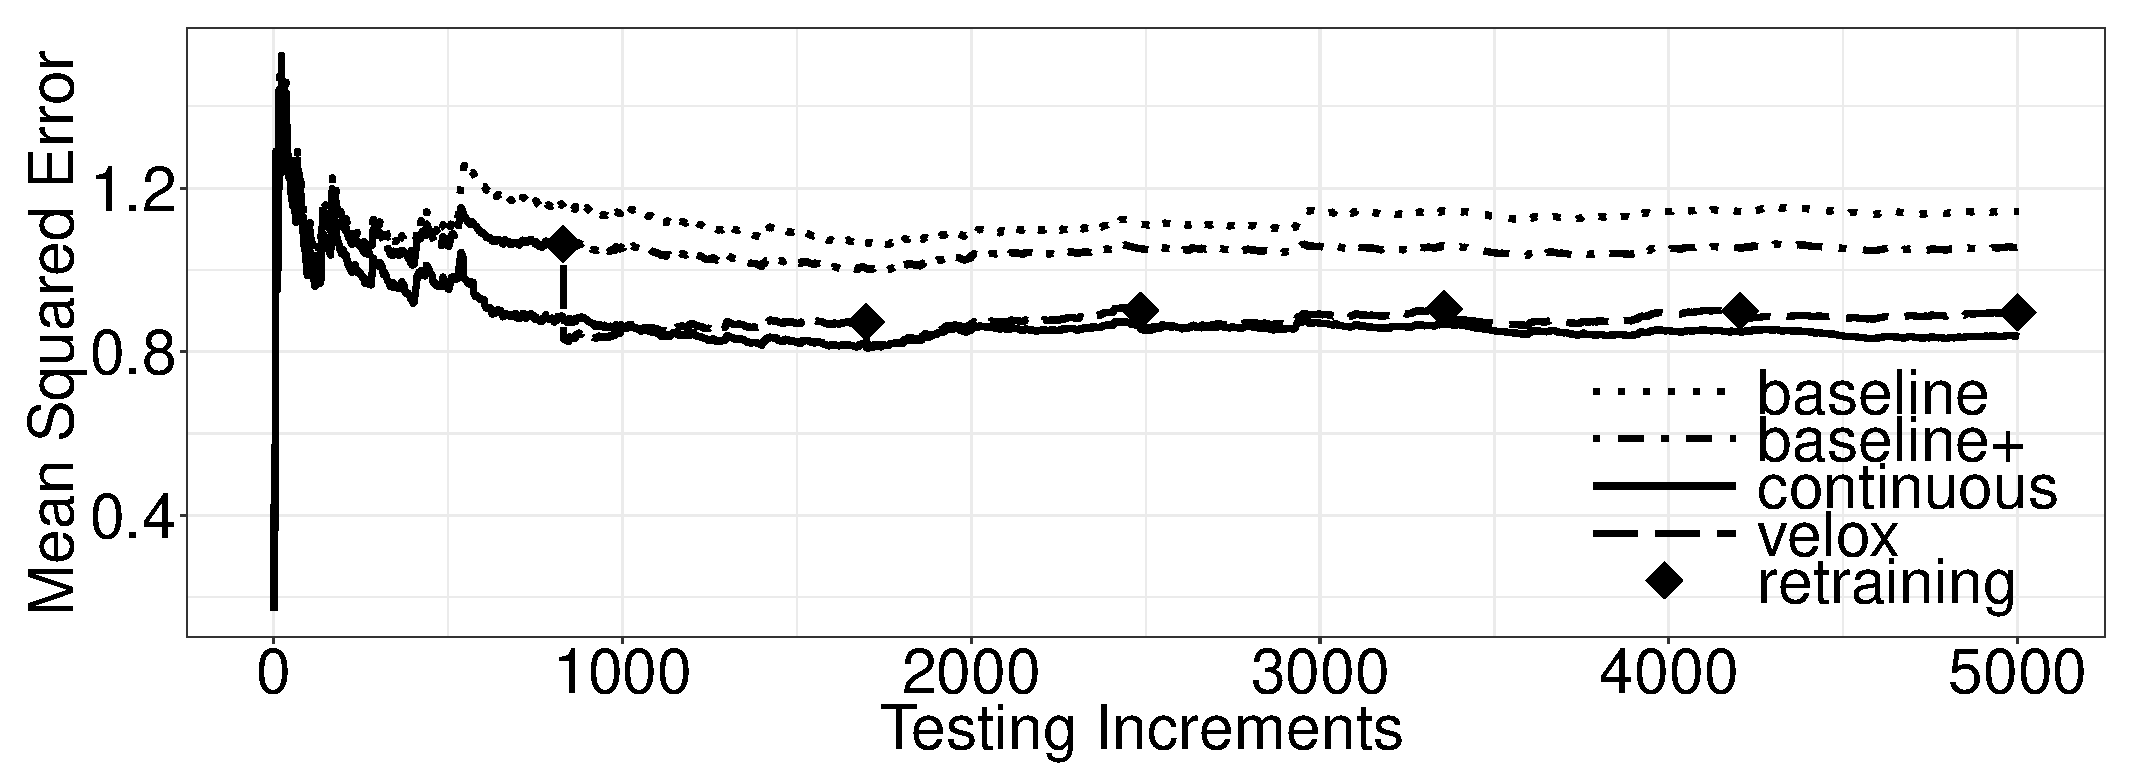
\includegraphics[width=\columnwidth]{../images/experiment-results/movie-lens-100k-quality-improved.eps}
	\caption{Movie Lens 100k}
	\label{fig:movie-lens-100k-score}
\end{subfigure}
\begin{subfigure}{\columnwidth}
  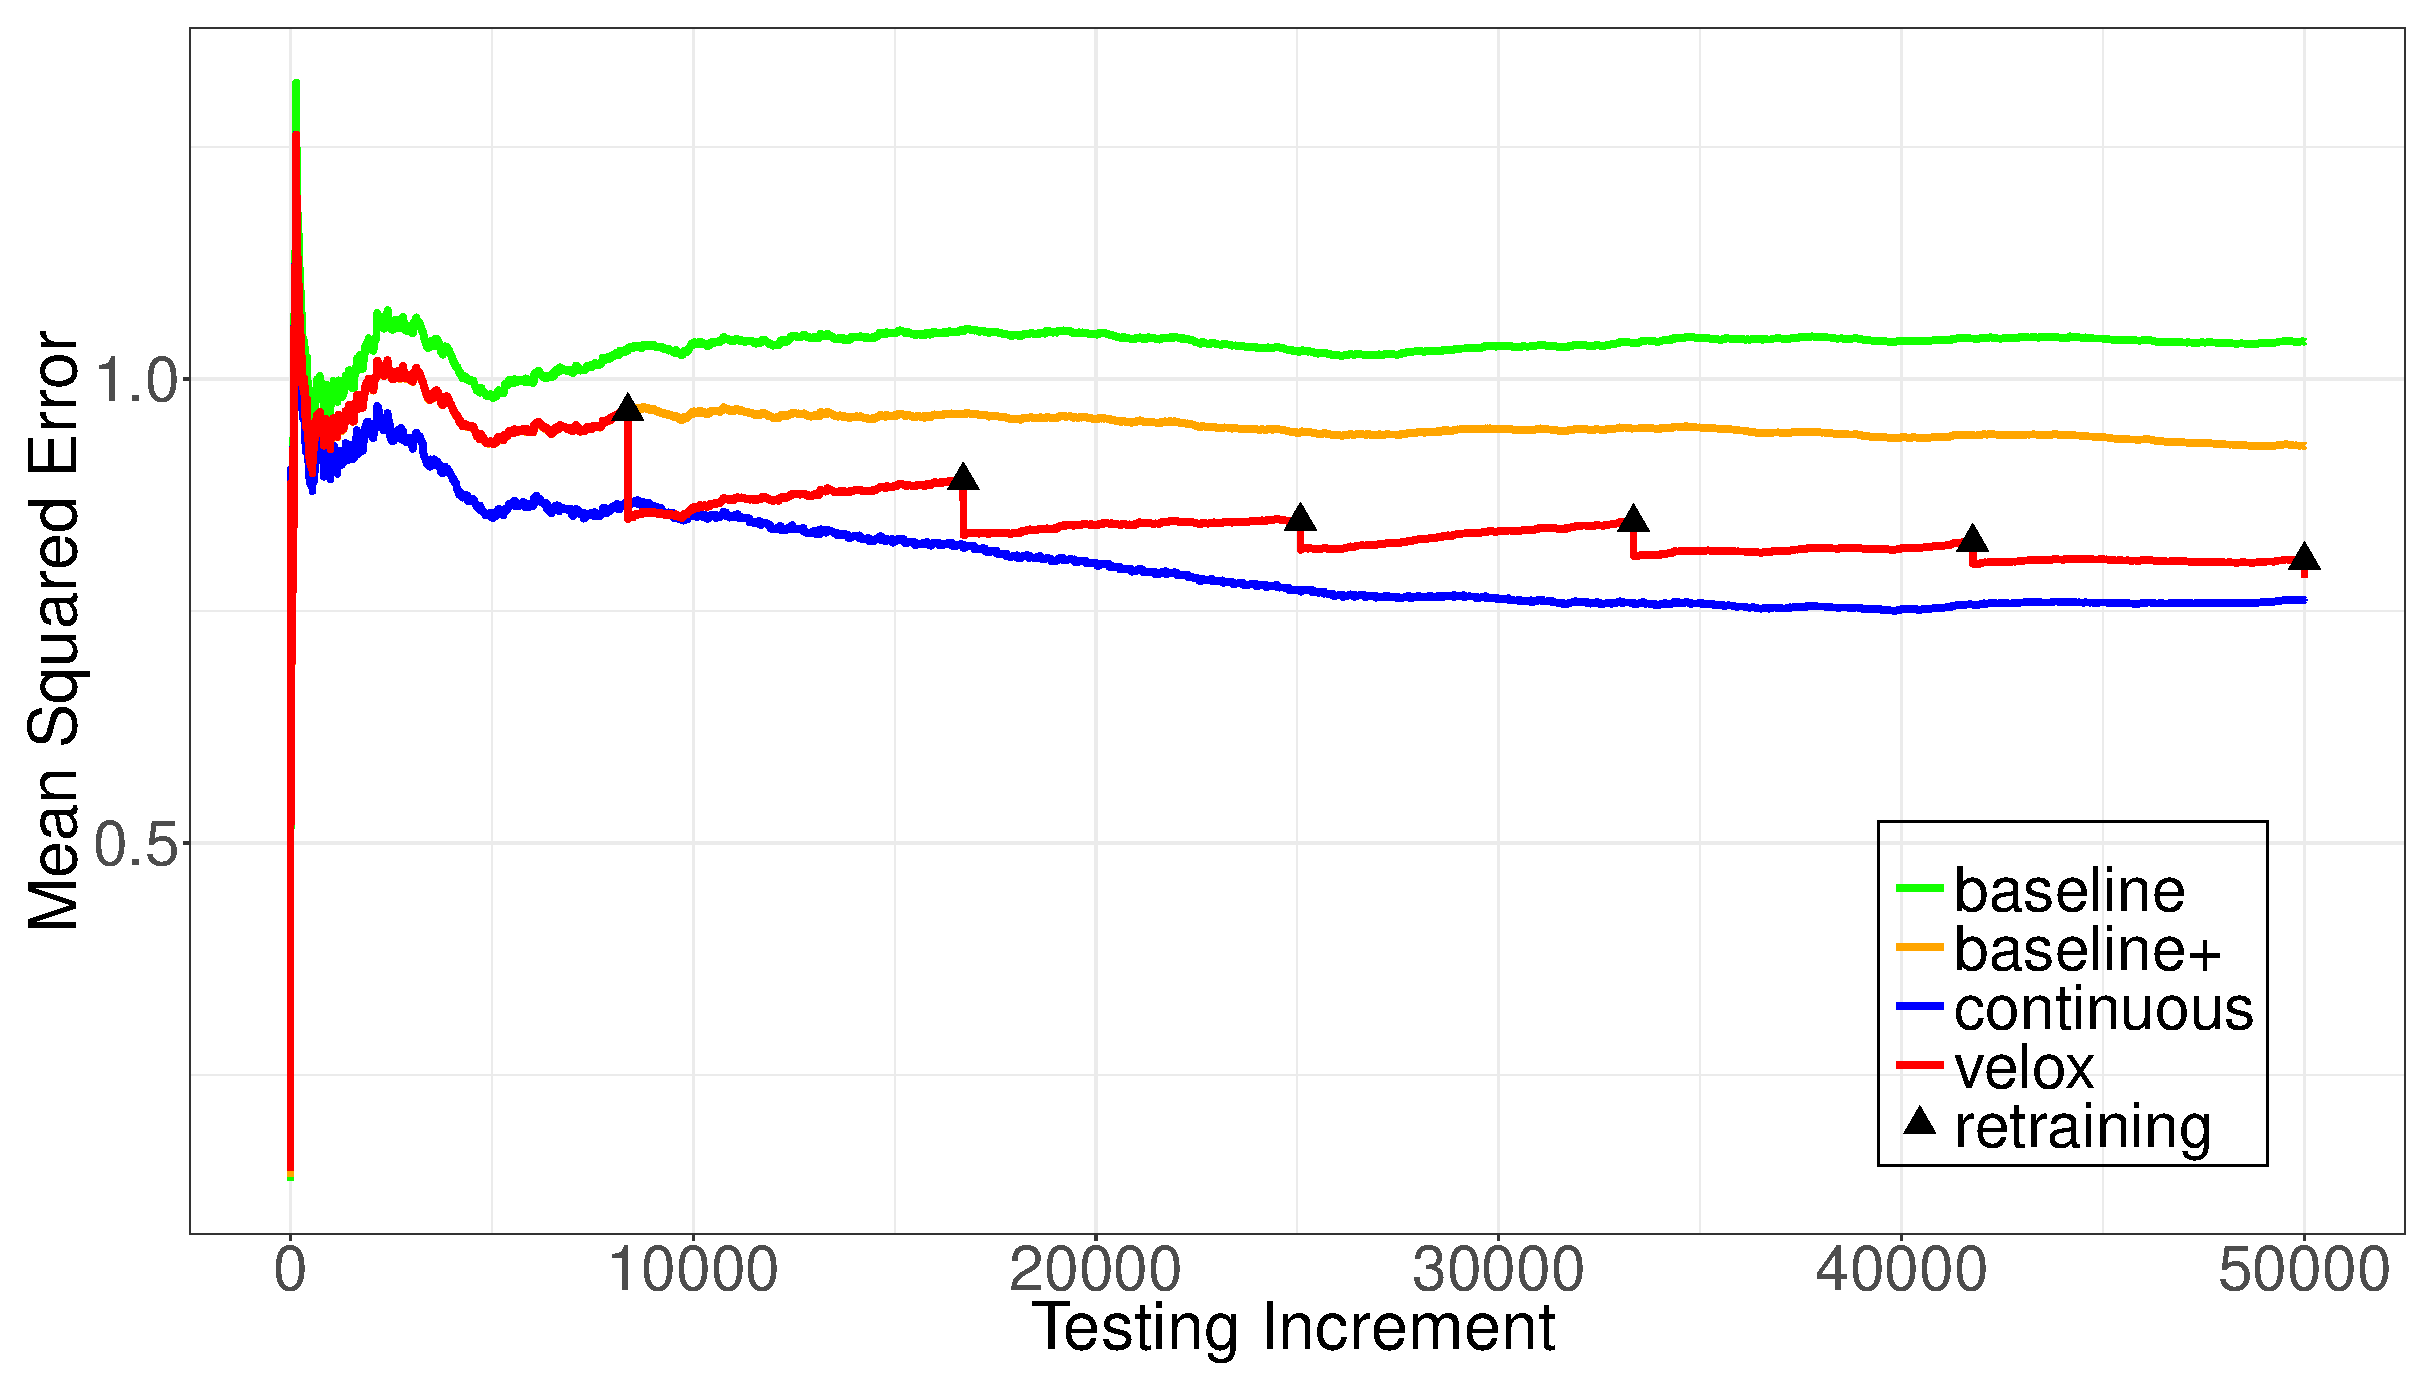
\includegraphics[width=\columnwidth]{../images/experiment-results/movie-lens-1m-quality-improved.eps}
\caption{Movie Lens 1M}
\label{fig:movie-lens-1M-score}
\end{subfigure}
\vspace{2mm}
\caption{Recommender Systems}
\end{figure}

Figure \ref{fig:movie-lens-100k-score} shows the mean squared error of Continuous, Velox, Baseline+, and Baseline on Movie Lens 100k dataset.
The scheduling rate (buffer size) is set to 500 for Continuous and 15,000 for Velox.
All four methods perform an initial training, therefore they have similar error rates in the beginning.
However, the error rate of Baseline starts to increase since it does not incrementally update the model.
Baseline+ incrementally updates the model.
As a result, it has a lower error rate than Baseline.
The error rate of Velox is similar to Baseline+ until the first scheduled retraining for Velox.
After the retraining, there is a sudden drop in the error rate.
For the remainder of the data, Velox performs as expected, once there is a retraining, the error rate immediately decreases.
This decrease in error rate is followed by a slow increase due the fact that Velox only incrementally updates the model until the next scheduled retraining, which as discussed earlier is not handling the change in the data distribution gracefully.
Initial error rate of Continuous is similar to the other methods.
However, the error rate starts to decrease rapidly.
The reason for the fast decrease in error rate is that immediately after the deployment of the model, the Continuous method executes iterations of SGD.
It consistently manages to adopt to the changes in data and decreases the error rate.
As expected, except for immediately after a full retraining, Continuous always performs better than Velox.

Figure \ref{fig:movie-lens-1M-score} shows the mean squared error rate achieved by the implemented methods on Movie Lens 1M.
Similar to Movie Lens 100k, Continuous has the lowest error rate among all the implemented methods.
The difference in error rate between Continuous and Velox is even greater than the error rate for Movie Lens 100k.
This is because the change in data distribution in Movie Lens 1M is greater than Movie Lens 100k (data in Movie Lens 1M is gathered from a longer period of time).
Since Continuous adapts to the changes in distribution faster than Velox, it maintains a lower error rate throughout.
The error rate of Velox follows the same trend as in the case of Movie Lens 100k. 
After every retraining, the error rate first drops then slowly increases until the next retraining.
Similar to Movie Lens 100k dataset, the error rate of Baseline is the highest among all the implemented methods, followed by Baseline+ , where due to the incremental updates of the model the error rate is lower.

\begin{figure}[h]
	\centering
\begin{subfigure}[b]{\columnwidth}
	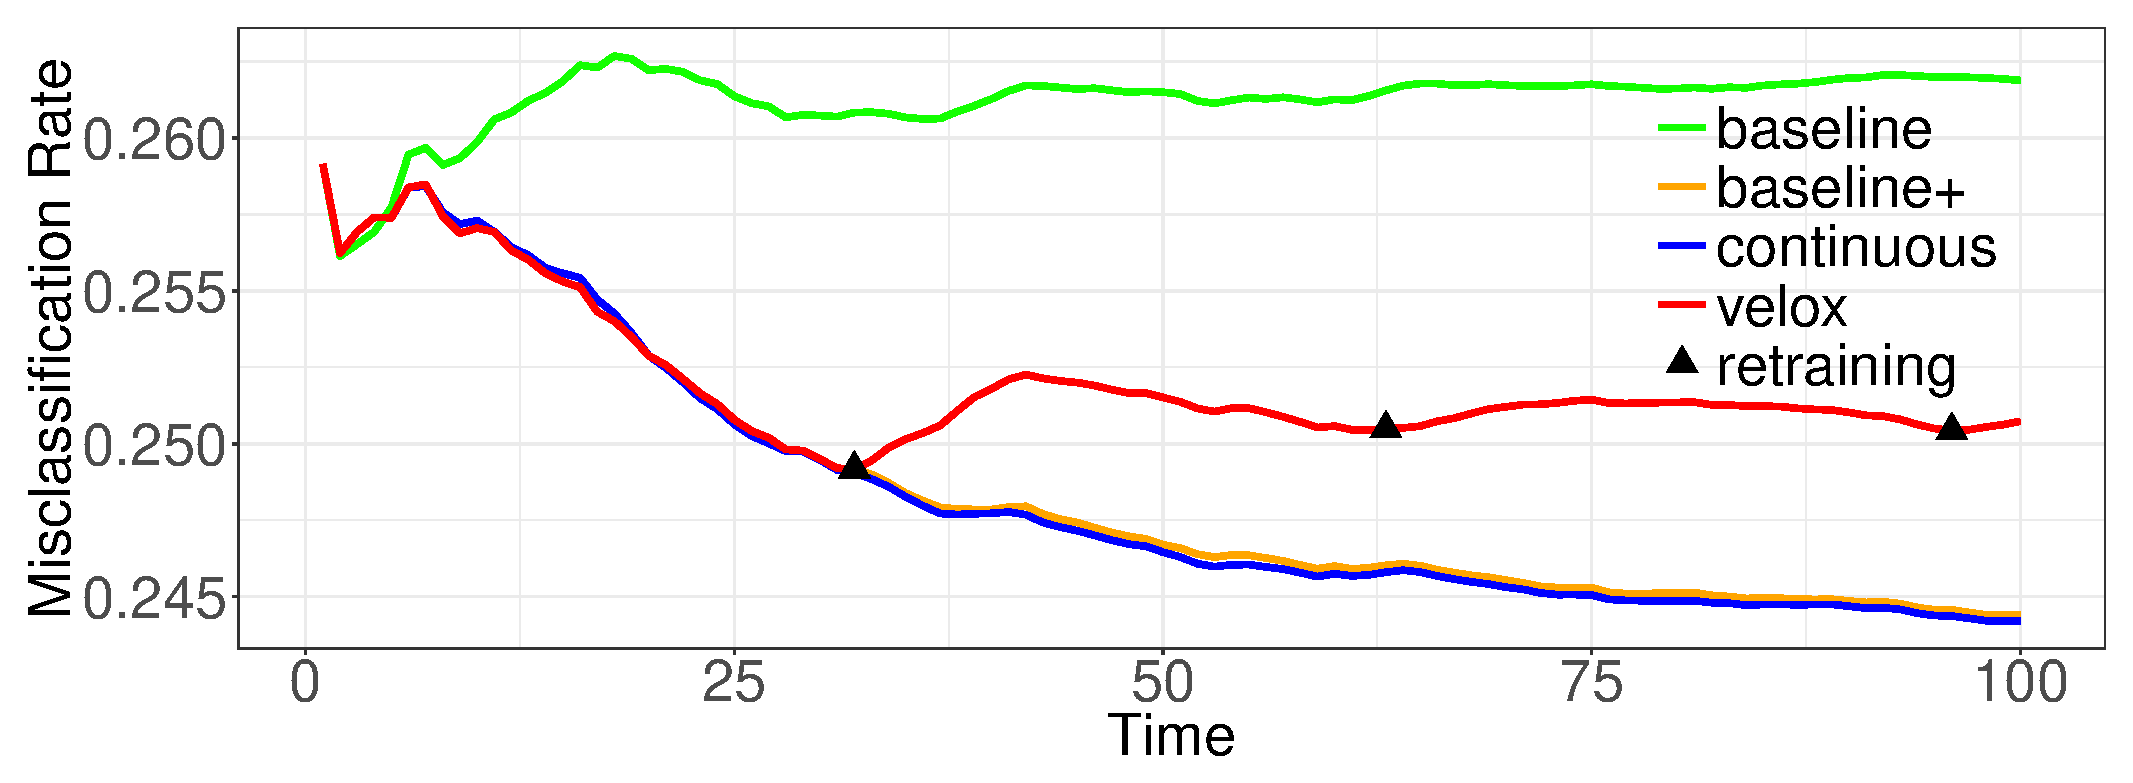
\includegraphics[width=\columnwidth]{../images/experiment-results/cover-types-quality.eps}
	\caption{Cover Types}
	\label{fig:cover-types-quality}
\end{subfigure}
\begin{subfigure}[b]{\columnwidth}
  	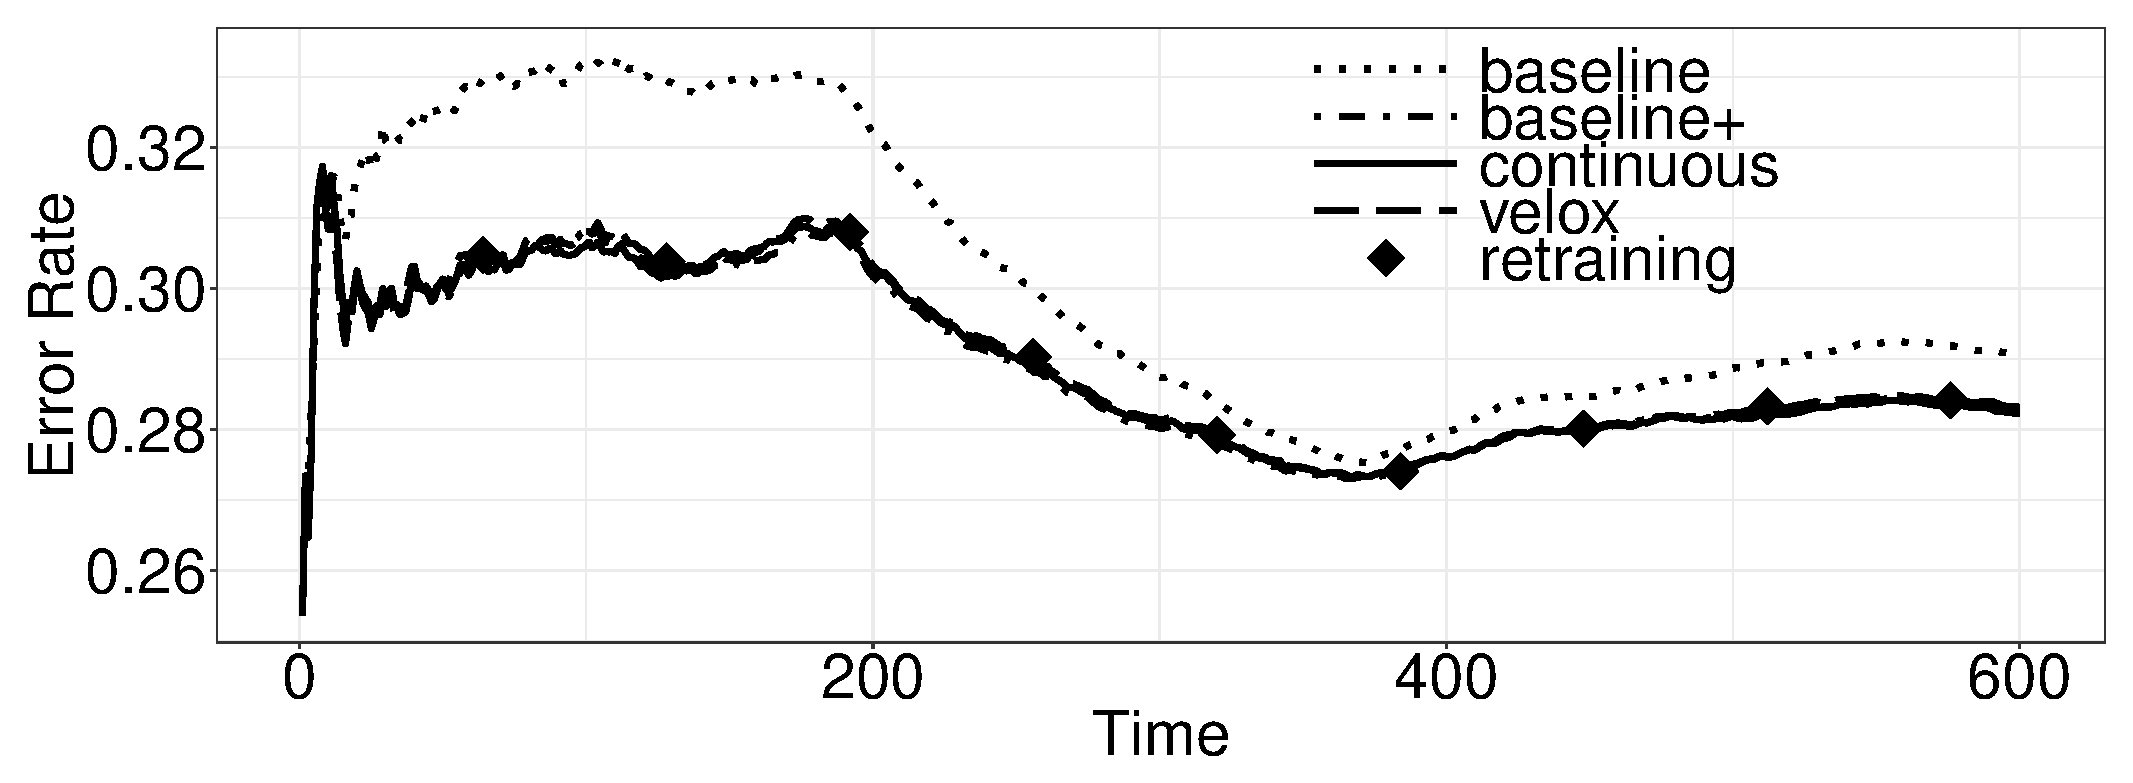
\includegraphics[width=\columnwidth]{../images/experiment-results/sea-quality.eps}
	\caption{SEA}
	\label{fig:sea-quality}
\end{subfigure}
\begin{subfigure}[b]{\columnwidth}
  	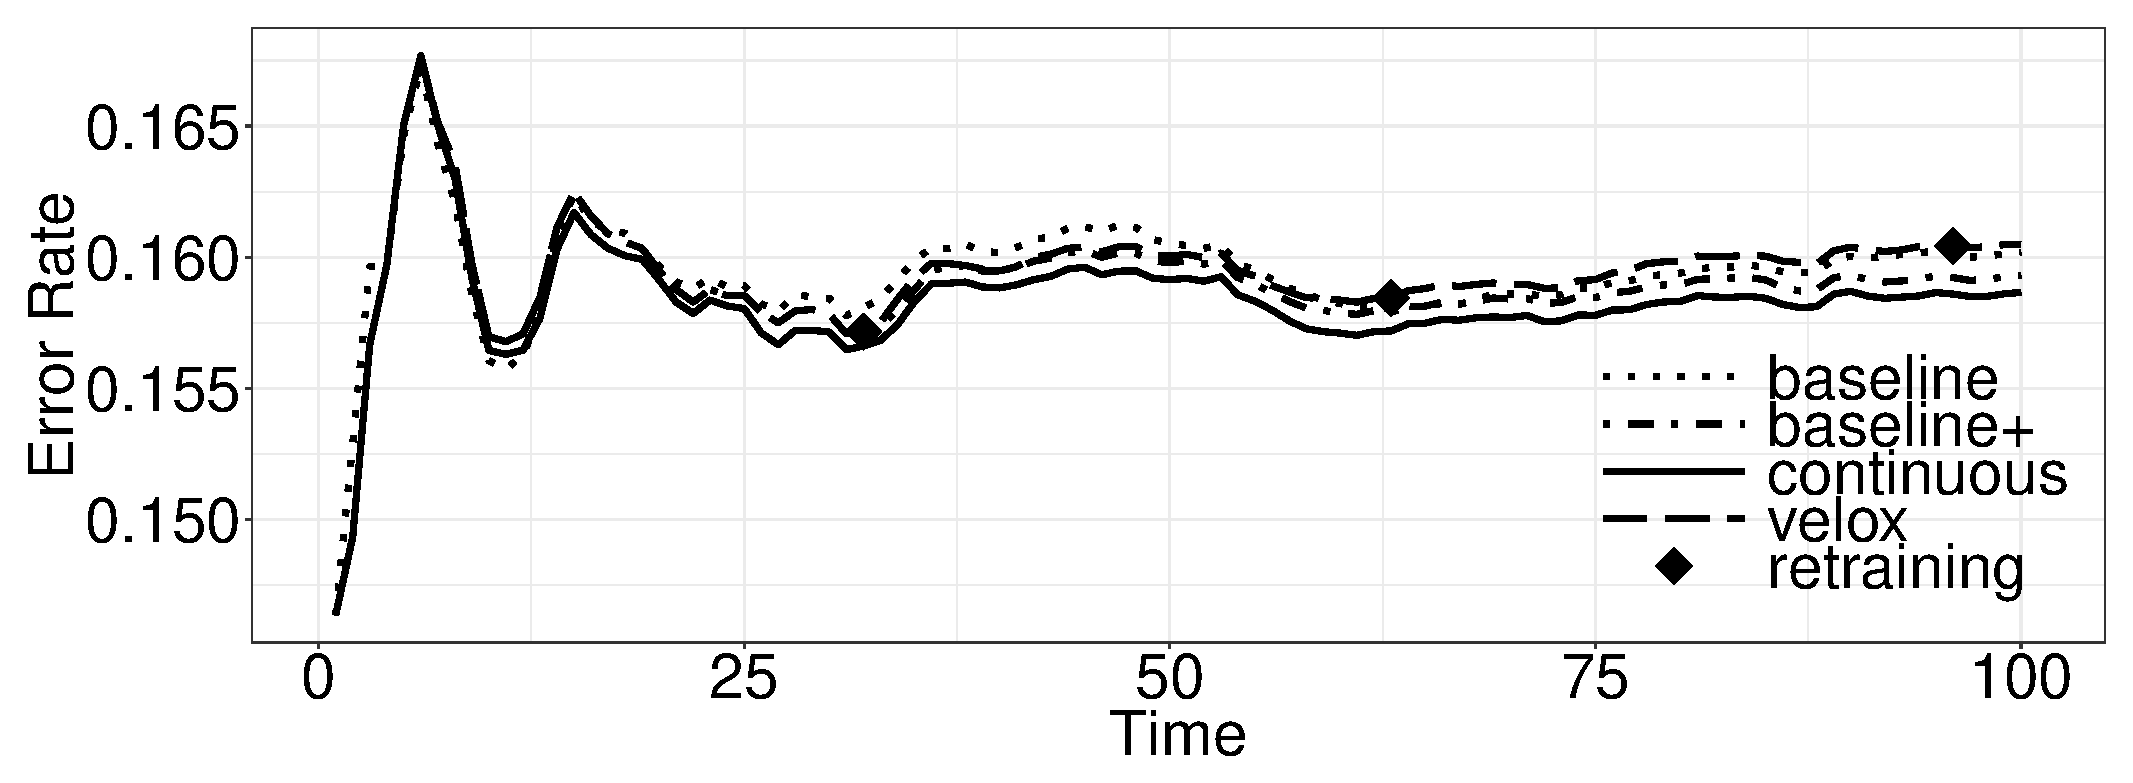
\includegraphics[width=\columnwidth]{../images/experiment-results/adult-quality.eps}
	\caption{Adult}
	\label{fig:adult-quality}
\end{subfigure}
\vspace{2mm}
\caption{Classification Datasets }
\label{fig:local-classification-results}
\end{figure}

Figure \ref{fig:local-classification-results} shows the misclassification rate over time for the implemented deployment methods on several classification datasets.
For all of the datasets, the sampling rate of Continuous is set to 0.2.
Contrary to the recommender system use case, the data used in these experiments is not time dependent (except for SEA) and as a result the deployment methods behave differently.
For Cover type (Figure \ref{fig:cover-types-quality}), Continuous achieves the lowest error rate overall, followed by Baseline+.
Baseline method has the highest error rate because it is not performing incremental updates on the model.
The error rate of Velox slightly increases after the first retraining and it never recovers from this increase.
By performing a retraining, the underlying model in Velox overfits to the existing data, therefore the test error on incoming data does not decrease the same way that it does in case of Baseline+ and Continuous.
The error rate for all of the deployment methods, except for Baseline is very similar on SEA (Figure \ref{fig:sea-quality}).
Continuous still perform slightly better than Baseline+ and Velox, although with a very small margin.
Figure \ref{fig:adult-quality} shows the error rate of different deployment methods on Adult dataset.
In this dataset, the different deployment methods perform rather similarly.
Baseline has the highest error rate overall, however after the 4th retraining the difference between the error rate of Velox and Baseline becomes smaller.
This is, similar to the Cover types dataset, due to the over training of the underlying model in Velox.
Baseline+ and Continuous maintain a steady error rate overall, with Continuous slightly outperforming Baseline+.

\begin{figure*}[h]
\begin{subfigure}[b]{0.2\textwidth}
	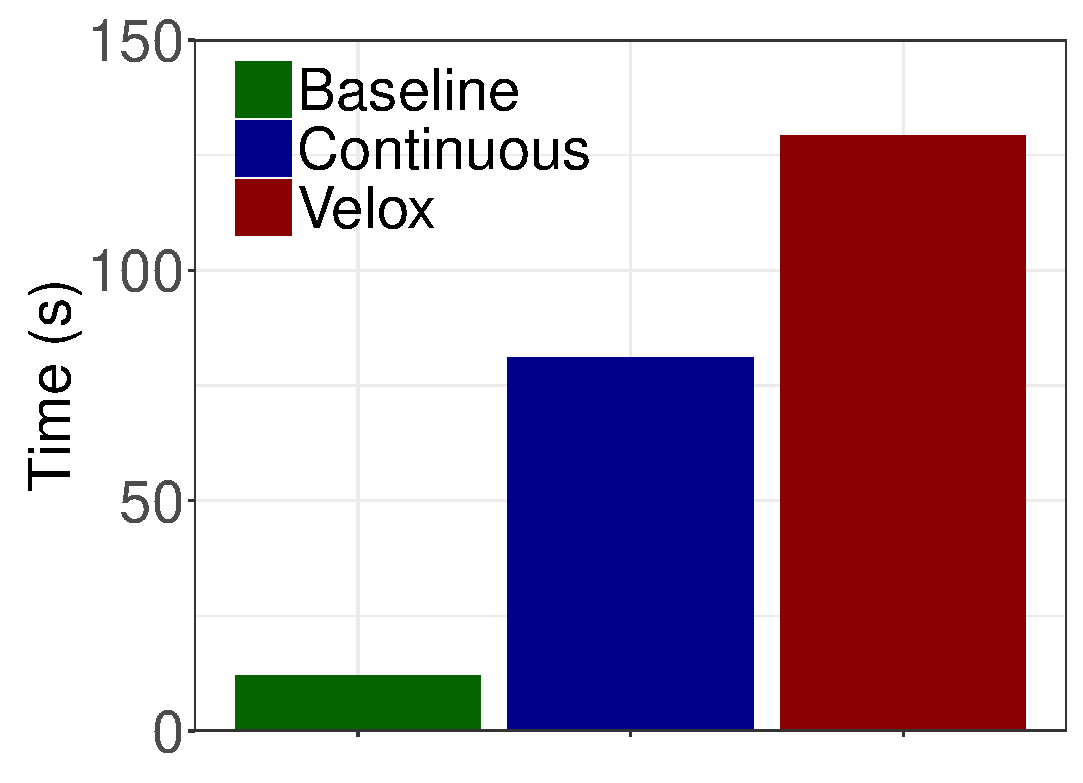
\includegraphics[width=\linewidth, height=\linewidth,keepaspectratio]{../images/experiment-results/cover-types-times.eps}
	\caption{Cover Types}
	\label{fig:cover-types-times}
\end{subfigure}%
\begin{subfigure}[b]{0.2\textwidth}
	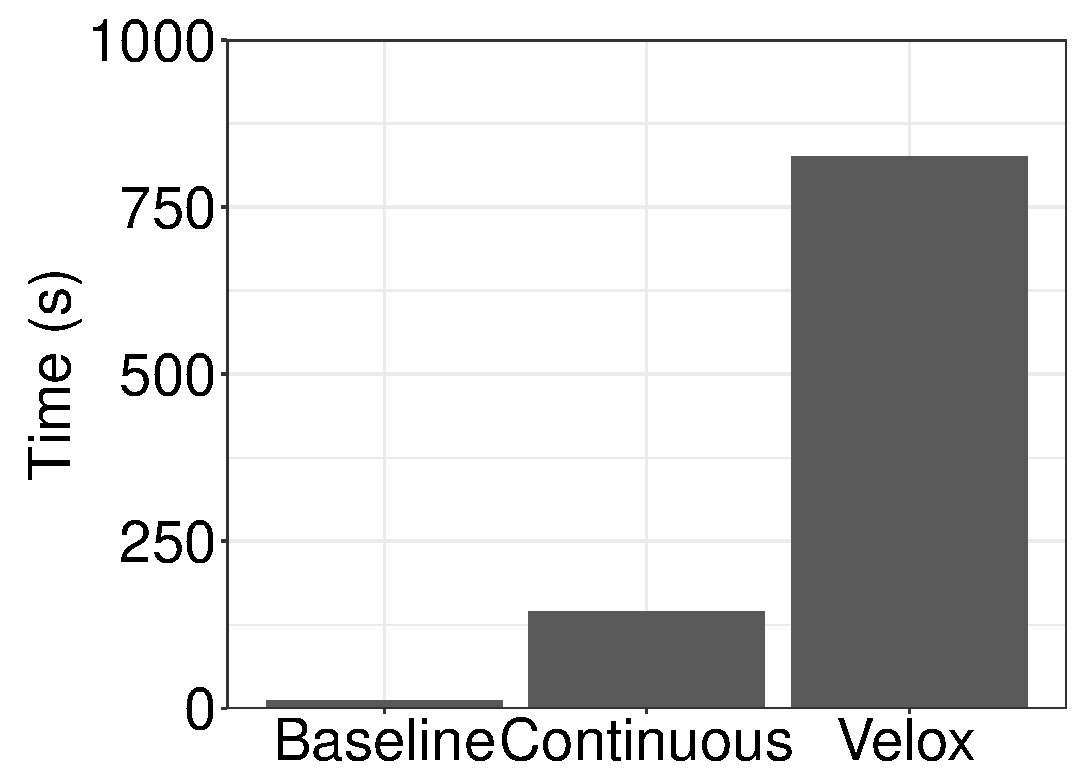
\includegraphics[width=\linewidth, height=\linewidth,keepaspectratio]{../images/experiment-results/sea-times.eps}
	\caption{SEA}
	\label{fig:sea-times}
\end{subfigure}%
\begin{subfigure}[b]{0.2\textwidth}
	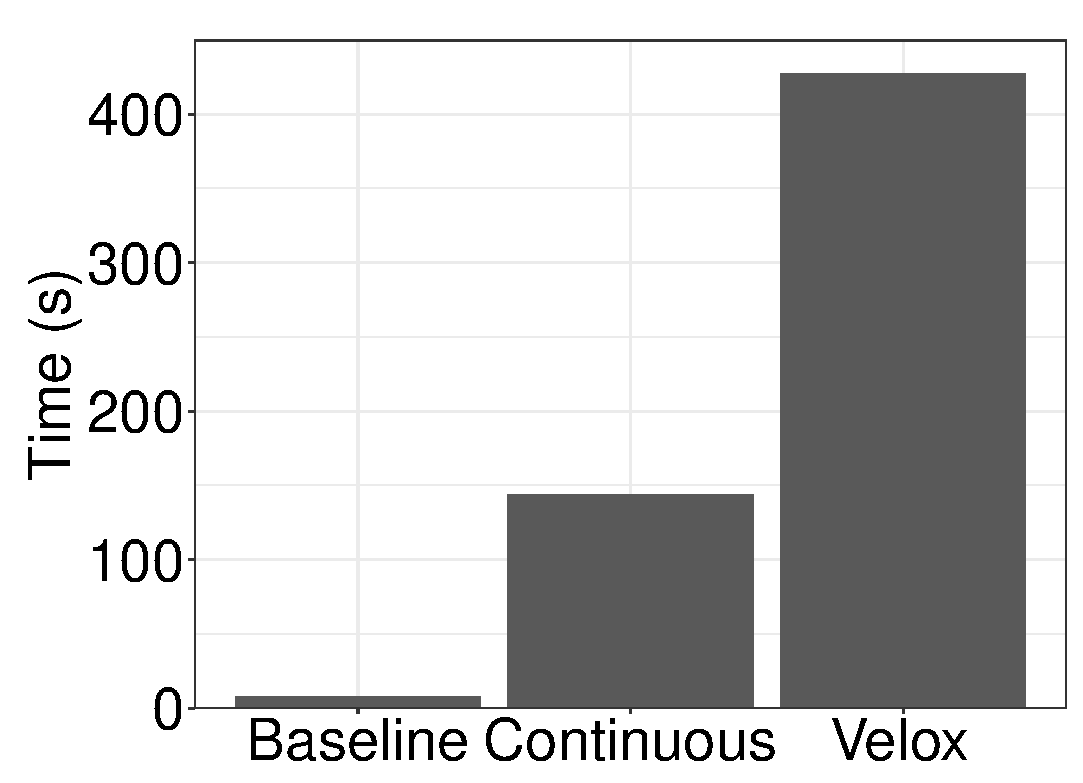
\includegraphics[width=\linewidth, height=\linewidth,keepaspectratio]{../images/experiment-results/adult-times.eps}
	\caption{Adult}
	\label{fig:adult-times}
\end{subfigure}%
\begin{subfigure}[b]{0.2\textwidth}
	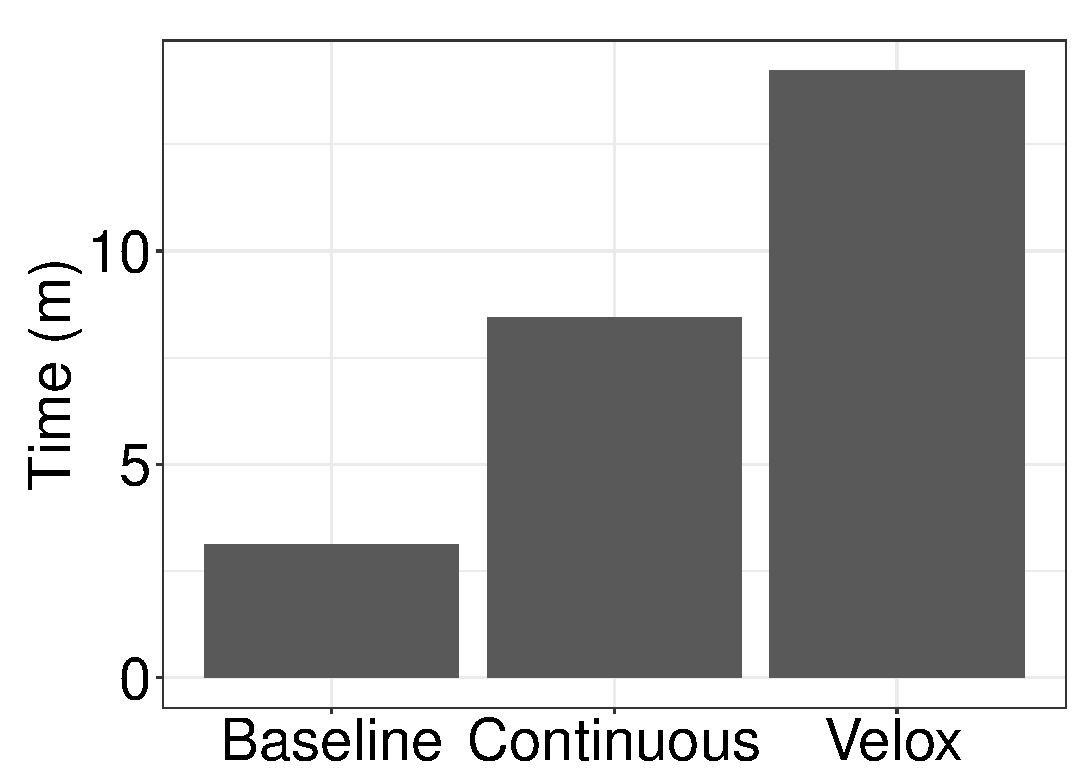
\includegraphics[width=\linewidth, height=\linewidth,keepaspectratio]{../images/experiment-results/movie-lens-100k-times.eps}
	\caption{Movie Lens 100k}
	\label{fig:movie-lens-100k-times}
\end{subfigure}%
\begin{subfigure}[b]{0.2\textwidth}
  	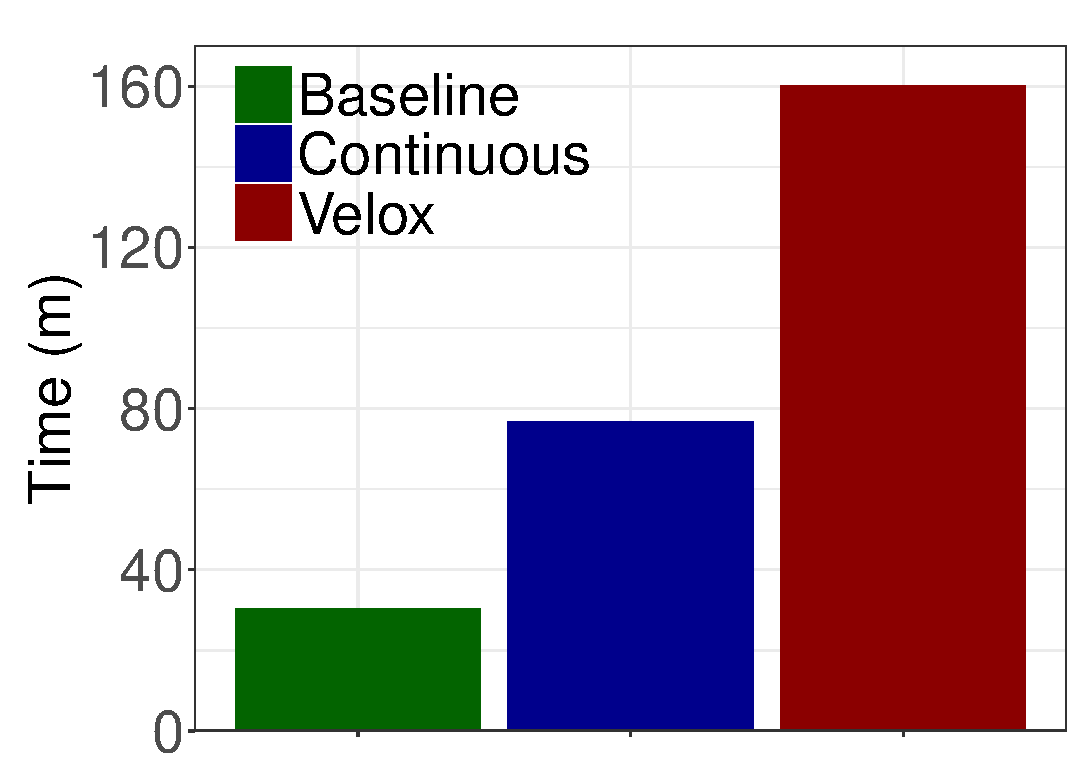
\includegraphics[width=\linewidth, height=\linewidth,keepaspectratio]{../images/experiment-results/movie-lens-1M-times.eps}
	\caption{Movie Lens 1M}
	\label{fig:movie-lens-1M-times}
\end{subfigure}%
\vspace{2mm}
\caption{Total training time for Local Datasets}
 \label{fig:local-training-time}
\end{figure*}

Figure \ref{fig:local-training-time} shows the total training time for deployment methods on local datasets.
To measure this value, we calculated the total time that each method spent in training the model.
We excluded the incremental training time as both Velox and Continuous perform incremental training as part of their process.
The total training time of Baseline is equal to the initial training time.
Both Continuous and Velox perform the same initial training, as a result, their total training time cannot be smaller than Baseline.
For the classification datasets (Figure \ref{fig:cover-types-times}, {fig:sea-times}, {fig:adult-times}), Continuous and Velox are approximately 25 and 50 times slower than Baseline method.
This is expected, as both the amount of data and the frequency of training is much smaller for Baseline.
For recommender system experiments, the difference in total training time is smaller.
In our python prototype, the entire dataset is first loaded into the memory and then it is streamed to the deployment system one by one.
As a result, both Continuous and Velox can train the model much faster.
In all of the evaluated datasets, the total training time of Continuous is 2 to 5 times smaller than that of Velox.
This is because a full retraining incurs a higher overhead than continuously training the method.
Another reason for the difference in training time is that as the size of the data increases, the time for running a new iteration in Continuous stays approximately the same, whereas the time for a full retraining increases exponentially.

\subsection{Experiments in the Distributed Environment}
We evaluated our deployment system on larger workloads in a distributed environment.
Figure \ref{fig:cluster-classification-results} shows the error rate of different deployment methods on classification datasets.
Since URL Reputation data was gathered over 120 days, it is very likely that the data contains changes in the distribution.
This concept drift is reflected in Figure \ref{fig:url-quality}.
The error rate of Baseline is increasing with a steady rate as it cannot adapt to the changes in the data.
Continuous achieves the lowest error rate overall.
Velox manages to keep the error rate lower than Baseline+ until the the second retraining, after which the error rate slightly increases. 
Figure \ref{fig:higgs-quality} shows the error rate on Higgs dataset.
Similar to local classification datasets, the error rate for Baseline is the highest among all of the deployment methods.
Velox, Baseline+, and Continuous maintain the same error rate until the first retraining of Velox, after which due to possible overfitting, the error rate of Velox slightly increases.
Continuous performs slightly better than Baseline+ in the beginning, however, the underlying models of both deployment methods slowly converges.
Therefore, the error rates of both of the deployment methods become similar.

\begin{figure}[h]
	\centering
\begin{subfigure}[b]{\columnwidth}
	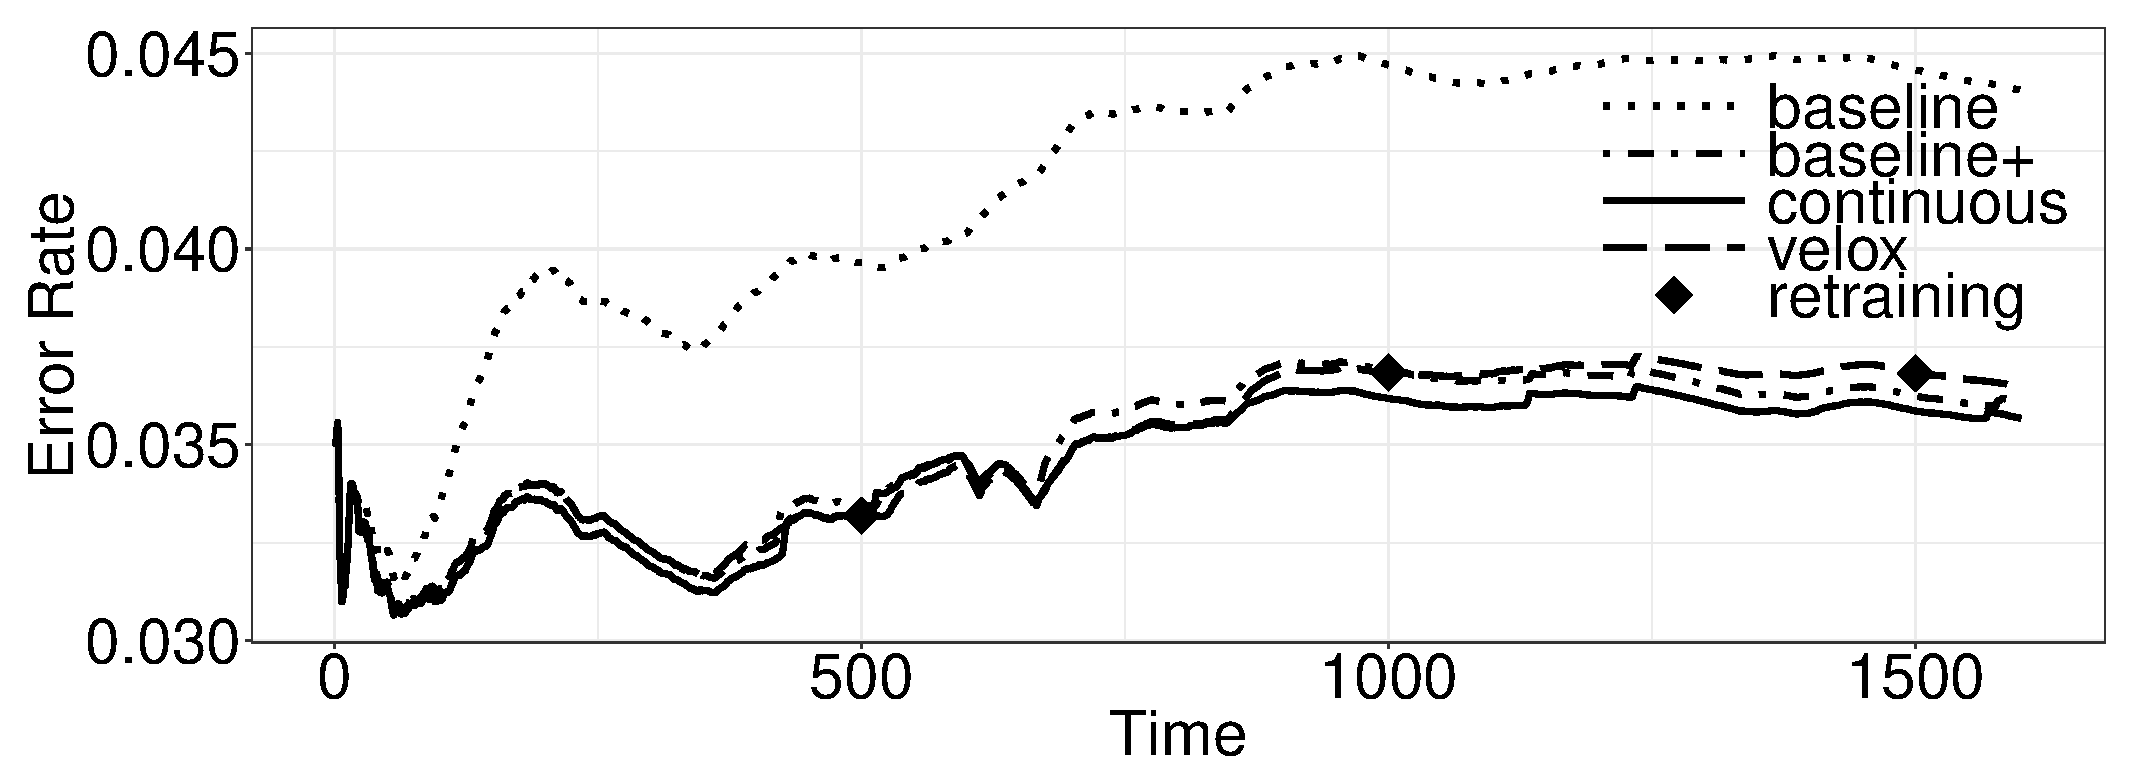
\includegraphics[width=\columnwidth,height=0.4\columnwidth]{../images/experiment-results/url-reputation-quality.eps}
	\caption{URL Reputation}
	\label{fig:url-quality}
\end{subfigure}
\begin{subfigure}[b]{\columnwidth}
  	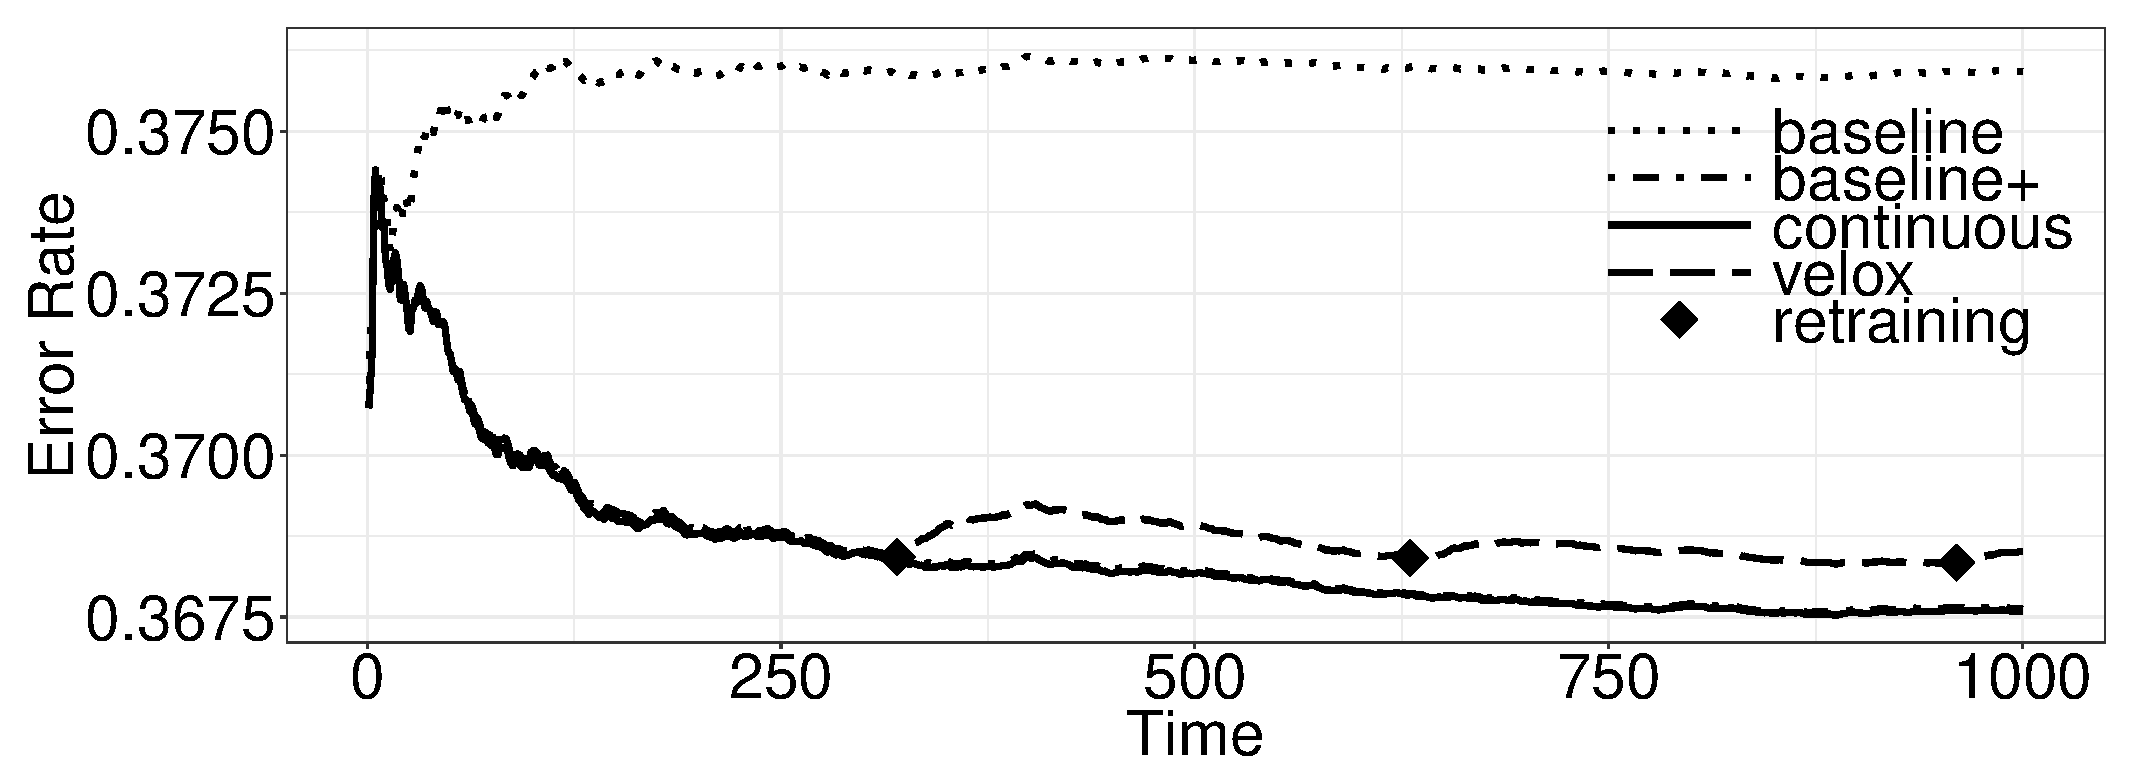
\includegraphics[width=\columnwidth,height=0.4\columnwidth]{../images/experiment-results/higgs-quality.eps}
	\caption{Higgs}
	\label{fig:higgs-quality}
\end{subfigure}
\vspace{2mm}
\caption{Large Classification Datasets}
\label{fig:cluster-classification-results}
\end{figure}


\begin{figure}[h]
\centering
\begin{subfigure}[b]{0.5\columnwidth}
	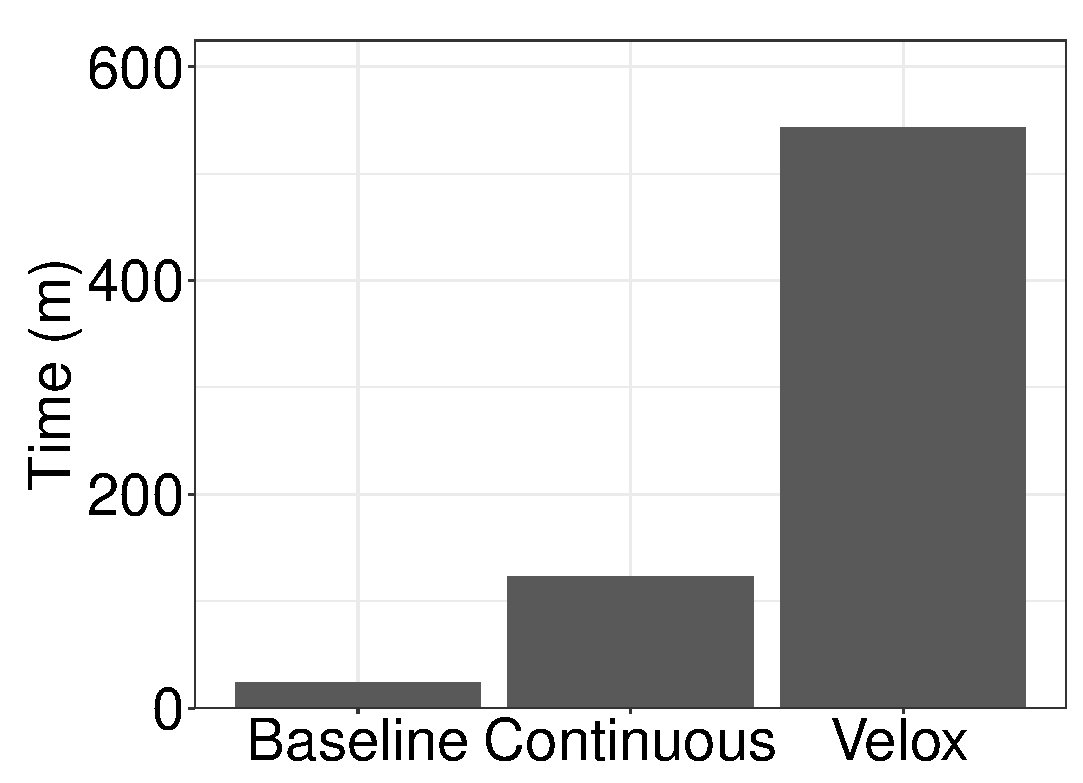
\includegraphics[width=\linewidth, height=\linewidth,keepaspectratio]{../images/experiment-results/url-reputation-times.eps}
	\caption{URL Reputation}
	\label{fig:url-times}
\end{subfigure}%
\begin{subfigure}[b]{0.5\columnwidth}
	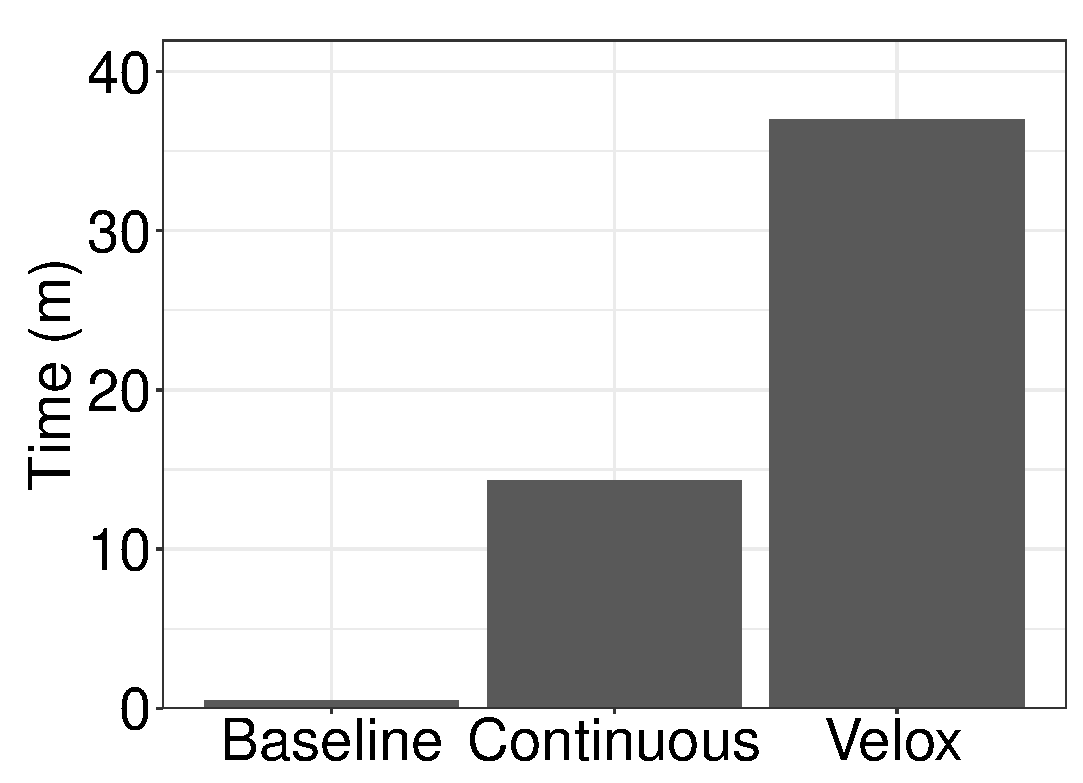
\includegraphics[width=\linewidth, height=\linewidth,keepaspectratio]{../images/experiment-results/higgs-times.eps}
	\caption{Higgs}
	\label{fig:higgs-times}
\end{subfigure}
\vspace{2mm}
\caption{Total training time for Distributed Datasets}
 \label{fig:cluster-training-time}
\end{figure}

Figure \ref{fig:cluster-training-time} shows the total training time for URL Reputation and Higgs experiments.
Similar to local datasets, Baseline has the smallest total training time.
However, the difference between the training time of Baseline and other methods is not as large.
In our local experiments, the entire resources of the computing machine was being consumed to perform the training.
However, in distributed environment, the cluster is underutilized in the beginning as the amount of data is small.
As more data arrives at the system, the utilization of the cluster increases.
As a result, the training time for Continuous and Velox does not increase linearly with size.
Therefore, the total training time for Continuous is only 5 to 10 times larger than that of Baseline (instead of 20 to 25 times for local datasets) and the total training time for Velox is 20 to 25 times larger than that of Baseline (instead of 50 to 55 times for local datasets).

\subsection{Discussion} \label{subsec:discussion}
\begin{figure*}[t]
\begin{subfigure}{0.30\textwidth}
  \centering
  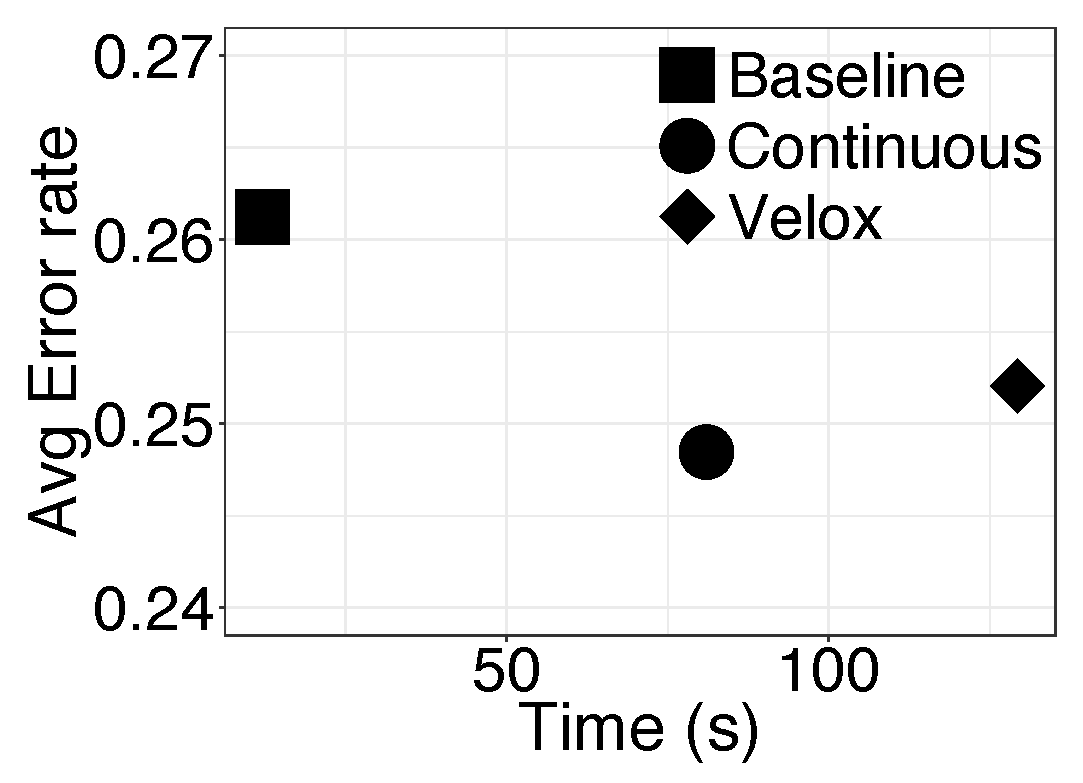
\includegraphics[width=\linewidth]{../images/experiment-results/cover-types-meta-performance.eps}
  \caption{Cover Type}
  \label{subfig:cover-type-meta}
\end{subfigure}%
  \hspace*{10mm}
\begin{subfigure}{0.30\textwidth}
 \centering
  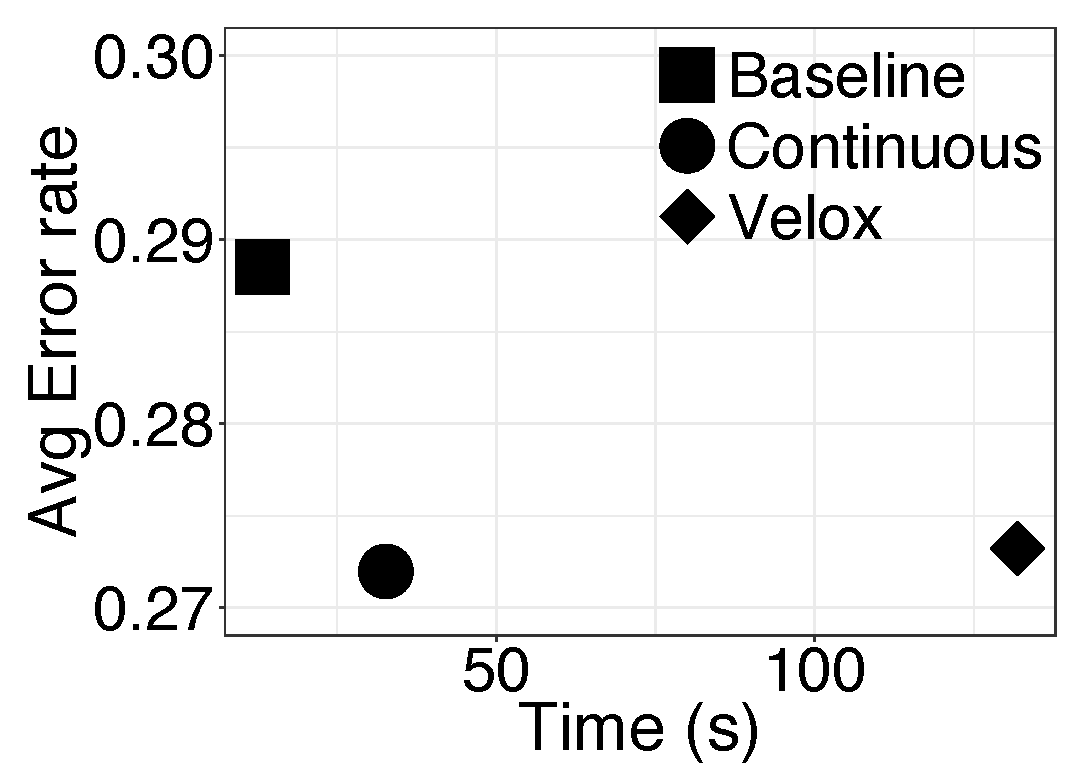
\includegraphics[width=\linewidth]{../images/experiment-results/sea-meta-performance.eps}
  \caption{SEA}
  \label{subfig:sea-meta}
\end{subfigure}%
 \hspace*{10mm}
 \begin{subfigure}{0.30\textwidth}
 \centering
  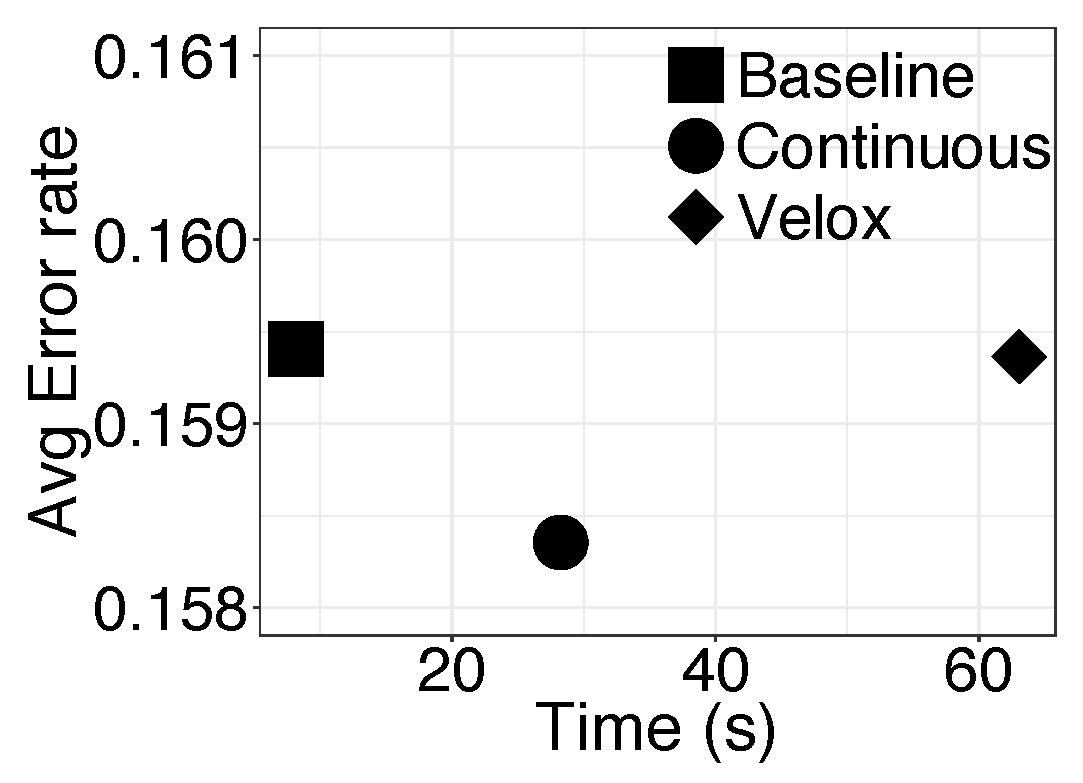
\includegraphics[width=\linewidth]{../images/experiment-results/adult-meta-performance.eps}
  \caption{Adult}
  \label{subfig:adult-meta}
\end{subfigure}%
 \vspace*{5mm}
\centering

\begin{subfigure}{.30\textwidth}
  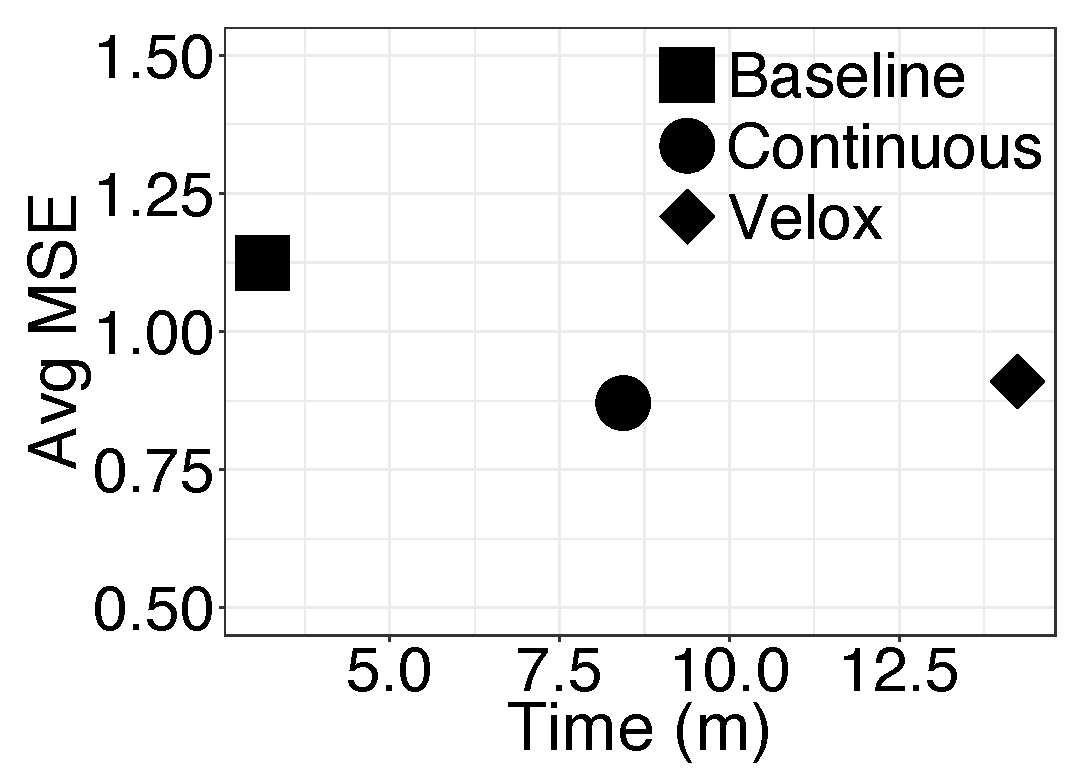
\includegraphics[width=1\linewidth, height=1\linewidth, keepaspectratio]{../images/experiment-results/movie-lens-100k-meta-performance.eps}
  \caption{Movie Lens 100K}
  \label{subfig:movie-lens-100k-meta}
\end{subfigure}%
 \hspace*{10mm}
\begin{subfigure}{0.30\textwidth}
  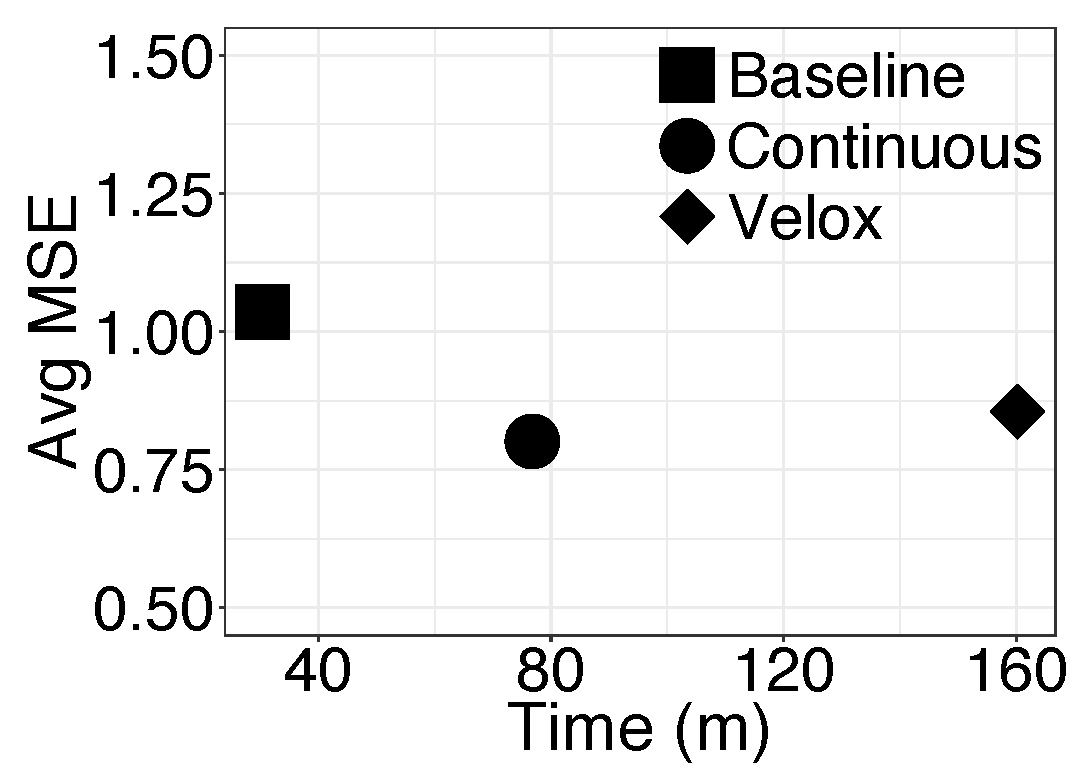
\includegraphics[width=1\linewidth, height=1\linewidth, keepaspectratio]{../images/experiment-results/movie-lens-1m-meta-performance.eps}
  \caption{Movie Lens 1M}
  \label{subfig:movie-lens-1m-meta}
\end{subfigure}


\begin{subfigure}{0.30\textwidth}
  \centering
  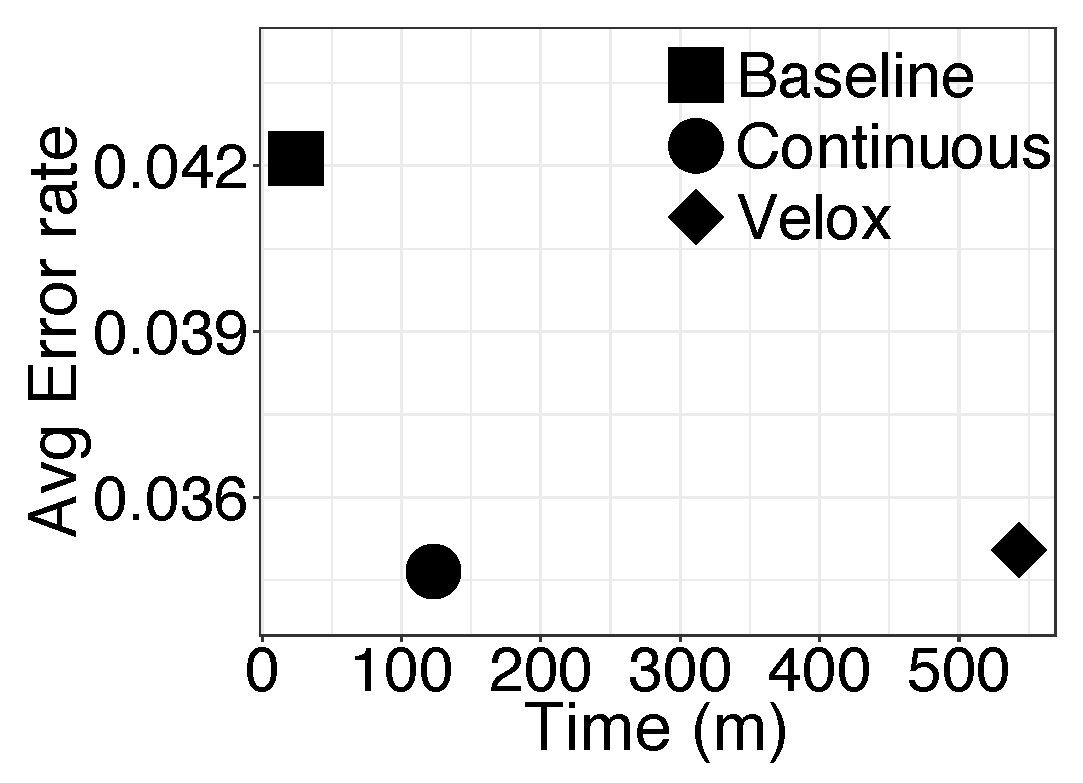
\includegraphics[width=\linewidth]{../images/experiment-results/url-reputation-meta-performance.eps}
  \caption{URL Reputation}
   \label{subfig:url-meta}
\end{subfigure}%
 \hspace*{10mm}
\begin{subfigure}{0.30\textwidth}
 \centering
  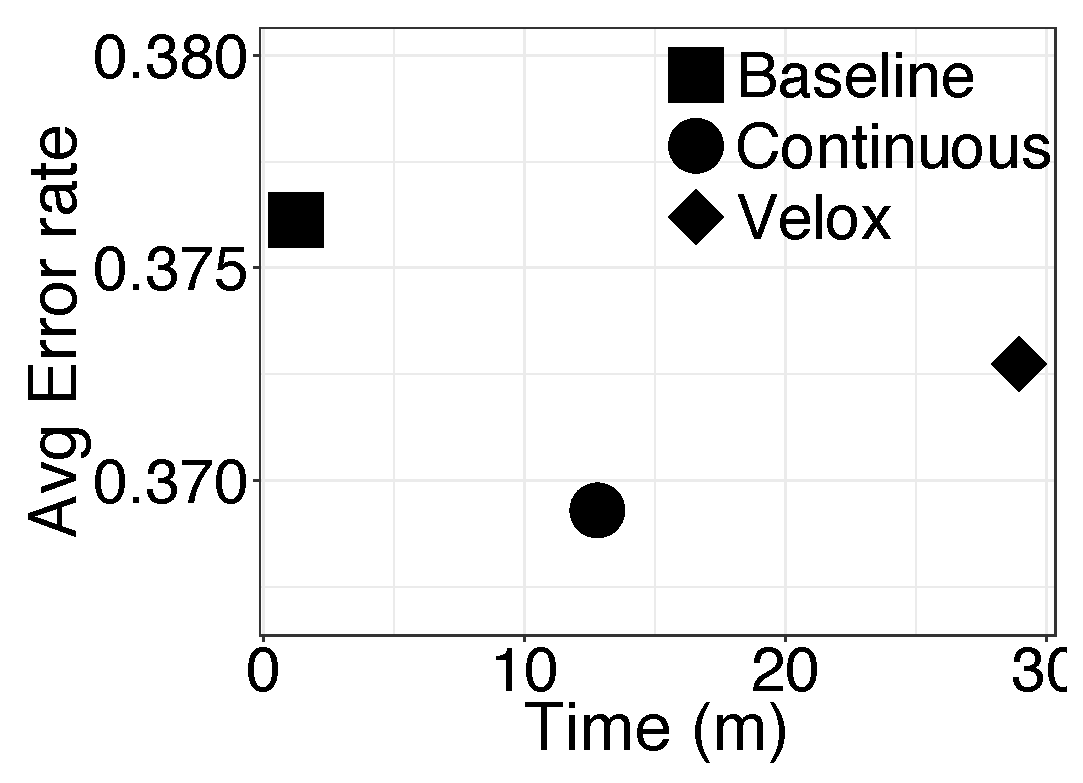
\includegraphics[width=\linewidth]{../images/experiment-results/higgs-meta-performance.eps}
  \caption{Higgs}
   \label{subfig:higgs-meta}
\end{subfigure}
 \vspace*{5mm}
\centering

\vspace{2mm}
\caption{Total Training Time vs Quality}
\label{fig:training-time-vs-quality}
\end{figure*}

Figure \ref{fig:training-time-vs-quality} shows the total training time and average error rate of each of the three different deployment methods (Baseline, Continuous, and Velox) on different datasets.
For all evaluated datasets, Continuous achieves the lowest average error rate (for classification datasets) and average mean squared error (for recommender system datasets).
The difference in average error rate (or average MSE) between Velox and Continuous is smaller for datasets that contain concept drift (Figure \ref{subfig:sea-meta}, \ref{subfig:movie-lens-100k-meta}, \ref{subfig:movie-lens-1m-meta}, and \ref{subfig:url-meta}).
Since both Velox and Continuous perform incremental training of the model after it is deployed, they both manage to handle the concept drift in the data.
However, Continuous is able to adapt to the changes faster as it is constantly updating the model by executing iterations of SGD.
In the deployment method of Velox, the underlying model cannot adapt to the changes in the distribution as quickly, since the retraining procedure cannot be executed frequently as it requires a lot of resources.
The performance of Baseline is very poor in datasets with concept drift.
This is expected, as the underlying model in Baseline is only trained on an initial dataset and is not able to adapt to the changes in the data.
Continuous performs very well for datasets with no concept drifts (Figure \ref{subfig:cover-type-meta},  \ref{subfig:adult-meta}, and \ref{subfig:higgs-meta}) as well.
For both Cover Type and Higgs datasets, Baseline method does not converge on the initial dataset, therefore it has a higher error rate than Velox and Continuous.
Velox performs better than Baseline on Higgs and Cover Type, however, retraining on these two datasets causes the underlying model to overfit to the existing data and as a result the performance of the model is decreased after each retraining.
This leads to an overall lower average error rate than that of Continuous

As expected, Baseline has the lowest training time for all the datasets since it only trains the model once on the initial datasets.
The total training time for Continuous is 2 to 5 time smaller than Velox for every datasets.
This has a big impact on prediction latency and prediction accuracy.
In our current prototype, we do not address the problem of the trade off between prediction latency and prediction accuracy.
In our prototype, both prediction and model updates are managed by the same node.
As a result the prediction component is paused until the SGD iteration (or retraining in the case of Velox) is executed.
Therefore, the system always answers each prediction query using the latest model, although with a much greater delay.
However, in an actual model deployment system, model training and prediction answering are typically executed on separate nodes (or threads), therefore any prediction request arriving at the system is answered immediately, although not with the latest version of the model.
Since the retraining time for Velox is large, a considerable percentage of prediction requests are always answered by an older version of the model.
Therefore, while the system is executing a retraining, the error rate of the answered prediction requests will continue to rise until the retraining is finished.
For example in URL Reputation dataset, the average time of each retraining is 68 minutes in Velox, whereas the average time of each iteration of SGD is 1.5 minutes.
This means that in worst case scenario, the model that is answering a prediction request in Velox is outdated by 1 hour.
Our continuous deployment method reduces this delay since it is updating the underlying model constantly using smaller batches of data.

\section{Conclusions} \label{conclusion}
To fully benefit from machine learning models, one has to deploy them in a system capable of answering prediction queries in real-time and continuously update the models so they adjust to the changes in the incoming data.
To continuously update a model, existing deployment systems perform two types of updates to the model; incremental training and full retraining of the model.
However, full retraining is a resource intensive and time consuming process.

We propose a system for deploying and maintaining machine learning models that are trained using stochastic gradient descent optimization.
In our system, we schedule iterations of SGD to run while the machine learning model is answering prediction queries.
After every iteration, the model is updated with new parameters.
The frequent updates help in adapting the model to changes in the data distribution.
Moreover, our system is applicable to a wide range of machine learning models as demonstrated in our evaluation section.

Our experiments show that the continuous training of the machine learning models is much faster than full retraining, which is the most common approach in deployment and maintenance of machine learning models. 
We show that not only continuous training requires less resources but it also produces models with lower error rates that adapt to the changes in data faster.
Comparing to simple techniques such incremental learning or initial batch training, our technique produces a model with higher quality.

In future work, we will explore more advanced methods for sampling of historical data in order to investigate their effect on the performance of the system. Moreover, we plan to investigate the trade off between prediction latency and prediction accuracy.


\bibliographystyle{plain}

{\fontsize{8}{4}\selectfont \bibliography{main}}
\end{document}